\chapter*{Danksagung}

Ein besonderer Dank geb\"uhrt Ulli Kehrle. Ohne seine unerm\"udlichen Erklärungen
zum Thema \LaTeX{} und seine Hilfestellungen, auch in den späten Abendstunden,
w\"urde diese Dokumentation nicht in dieser Form existieren.

\newpage

\tableofcontents
\listoffigures
\begingroup
\let\clearpage\relax
\lstlistoflistings{}
%\listoftables
\endgroup


%% autogenerated by pandoc
%% we need to review this block

%\PassOptionsToPackage{unicode=true}{hyperref} % options for packages loaded elsewhere
%\PassOptionsToPackage{hyphens}{url}
%
%%\documentclass[]{article} % do we need that?
%%\usepackage{lmodern} % do we need that package?
%\usepackage{amssymb,amsmath}
%\usepackage{ifxetex,ifluatex}
%\usepackage{fixltx2e} % provides \textsubscript
%\ifnum 0\ifxetex 1\fi\ifluatex 1\fi=0 % if pdftex
%  \usepackage[T1]{fontenc}
%  \usepackage[utf8]{inputenc}
%  \usepackage{textcomp} % provides euro and other symbols
%\else % if luatex or xelatex
%  \usepackage{unicode-math}
%  \defaultfontfeatures{Ligatures=TeX,Scale=MatchLowercase}
%\fi
% use upquote if available, for straight quotes in verbatim environments
%\IfFileExists{upquote.sty}{\usepackage{upquote}}{}
% use microtype if available
%\IfFileExists{microtype.sty}{%
%\usepackage[]{microtype}
%\UseMicrotypeSet[protrusion]{basicmath} % disable protrusion for tt fonts
%}{}
%\IfFileExists{parskip.sty}{%
%\usepackage{parskip}
%}{% else
%\setlength{\parindent}{0pt}
%\setlength{\parskip}{6pt plus 2pt minus 1pt}
%}
%\usepackage{hyperref}
%\hypersetup{
%            pdfborder={0 0 0},
%            breaklinks=true}
%\urlstyle{same}  % don't use monospace font for urls
%\usepackage{longtable,booktabs}
% Fix footnotes in tables (requires footnote package)
%\IfFileExists{footnote.sty}{\usepackage{footnote}\makesavenoteenv{longtable}}{}
%\usepackage{graphicx,grffile}
%\makeatletter
%\def\maxwidth{\ifdim\Gin@nat@width>\linewidth\linewidth\else\Gin@nat@width\fi}
%\def\maxheight{\ifdim\Gin@nat@height>\textheight\textheight\else\Gin@nat@height\fi}
%\makeatother
% Scale images if necessary, so that they will not overflow the page
% margins by default, and it is still possible to overwrite the defaults
% using explicit options in \includegraphics[width, height, ...]{}
%\setkeys{Gin}{width=\maxwidth,height=\maxheight,keepaspectratio}
%\setlength{\emergencystretch}{3em}  % prevent overfull lines
%\providecommand{\tightlist}{%
%  \setlength{\itemsep}{0pt}\setlength{\parskip}{0pt}}
%\setcounter{secnumdepth}{0}
% Redefines (sub)paragraphs to behave more like sections
%\ifx\paragraph\undefined\else
%\let\oldparagraph\paragraph
%\renewcommand{\paragraph}[1]{\oldparagraph{#1}\mbox{}}
%\fi
%\ifx\subparagraph\undefined\else
%\let\oldsubparagraph\subparagraph
%\renewcommand{\subparagraph}[1]{\oldsubparagraph{#1}\mbox{}}
%\fi

% set default figure placement to htbp
%\makeatletter
%\def\fps@figure{htbp}
%\makeatother

\chapter{Vorwort}\label{vorwort}

Als Vorbereitung f\"ur die Abschlusspr\"ufungen im Juni 2018 haben die Sch\"uler der
Fachklassen des Heinrich\hyp{}Hertz\hyp{}Europakollegs Bonn ein Szenario in dem
Bereich der Serveradministration gestellt bekommen. Dieses wurde innerhalb
eines Teams von zwei bis zu drei Leuten eigenständig erarbeitet. Die Hardware,
worauf das Testszenario durchgef\"uhrt werden konnte, wurde von der Schule
gestellt. Den Sch\"ulern wurde freigestellt, ob Sie diese verwenden oder eigene
Mittel verwenden möchten.

Die Aufgabenstellung wurde \"uber Moodle zur Verf\"ugung gestellt und kann dem
Anhang~\ref{pdf:requirements} entnommen werden. Die Arbeit und das Verfassen
dieser Dokumentation wurde eigenständig durchgef\"uhrt.

\chapter{Vorbereitung}\label{vorbereitung}

Um eine vollständige und schnelle Umsetzung des Projektes zu gewährleisten
wurde zunächst eine Testumgebung aufgebaut. Des Weiteren wurde zu Beginn ein
Konzept erarbeitet, welches die DNS Namenkonvention und die DHCP Vorgaben
beinhaltet. Dieses Konzept wurde abschließend dem zuständigen Lehrer, in diesem
Projekt als Rolle des Auftraggebers, vorgelegt und abgenommen. Eine
vorausschauende Planung und Konzeptionierung zusammen mit dem Auftraggeber
bringt den Vorteil, dass Fehler fr\"uhzeitig identifiziert und verbessert werden
können, sowie eine effiziente Hardware Planung.

\section{DHCP-Konzept}\label{dhcp-konzept}

Die Firma Mikado besitzt insgesamt acht Abteilungen. Pro Abteilung wird ein
Netzwerkdrucker vorgesehen. Zum aktuellen Zeitpunkt verwendet die Firma ein
Class C Ipv4 Netz, welches beibehalten werden soll. Die Aufteilung der IP
Adressen f\"ur die Clients, sowie den Netzwerkdruckern, soll \"uber einen DHCP
Server vergeben werden. Dabei wird das folgende DHCP Konzept verwendet:

\begin{outline}
  \1 Jede Abteilung erhält einen eignen Adressbereich, in dem maximal 251
  Hosts verwendet werden können
  \1 Netzwerkdrucker erhalten den Ende eines jeden Netzwerkbereichs
\end{outline}

Der aktuelle Standard in der Wirtschaft ist aktuell, keine Subnetzmetze mit
einer Subnetzmaske kleiner 24 zu nutzen (Ausnahme sind Transfernetze).
Wird ein gr\"o\ss{}eresNetz ben\"otigt, so sollte es ein vielfaches eines Class
C Netz sein. Von den 256 Adressen entf\a"llt eine f\"ur die Broadcastadresse,
eine f\"ur die Netzadresse, eine f\"ur das Gateway und zwei f\"ur die VRRP
Adressen.
Die Aufteilung sieht anschließend wie folgt aus:

\begin{center}
  \begin{tabular}{lll}
    \toprule
    Abteilung                     & Netzadresse & Broadcastadresse  \\
    \midrule
    Leitung                       & 192.168.0.0 & 192.168.0.255     \\
    Einkauf                       & 192.168.2.0 & 192.168.2.255     \\
    Disposition                   & 192.168.3.0 & 192.168.3.255     \\
    Produktion                    & 192.168.4.0 & 192.168.4.255     \\
    Konstruktion                  & 192.168.5.0 & 192.168.5.255     \\
    Buchhaltung / Rechnungswesen  & 192.168.6.0 & 192.168.6.255     \\
    Verkauf                       & 192.168.7.0 & 192.168.7.255     \\
    \bottomrule
  \end{tabular}
  \captionof{table}{IP-Addressen Setup}
\end{center}

Die Rechner der Administratoren erhalten ein separates Netzwerk, in dem
ebenfalls die entsprechenden Windows Server vorhanden sein werden.

\section{DNS-Namensraum}\label{dns-namensraum}

Die Firma Mikado hat bereits den Domänennamen mikado.spiel erworben. Dieser
kann f\"ur die Domänen Struktur verwendet werden. \ mikado ist in diesem Fall die
Second-Level-Domain der DNS Namensauflösung und spiel die First-Level-Domain.
Es können weitere Subdomains (Third\hyp{}Level\hyp{}Domains) wie beispielsweise
verkauf, konstruktion oder einkauf hinzugef\"ugt werden. Die DNS Namensauflösung
ist f\"ur die Auflösung von FQDNs in eine IP Adresse und umgekehrt. Jeder
Rechnername in der internen Domäne ist ebenfalls im DNS eingetragen und kann
von diesem aufgelöst werden. Der Windows Server 2016, welcher den Domain
Controller besitzt, ist gleichzeitig auch ein DNS Server. Dadurch k\"onnen die
entsprechenden Einträge unmittelbar durch den Domain Controller an den DNS
Server weitergeben werden. Die Auflösung der IP Adresse, bei diesem Server dann
wie folgt:

W16dc01.mikado.spiel

\section{Windows Domänen Konzept}\label{windows-domuxe4nen-konzept}

\subsection{Namenskonzept User}\label{namenskonzept-user}

Um eine Eindeutigkeit der User herzustellen, empfiehlt es sich hier die
Personalnummer des Anwenders zu verwenden. Innerhalb der AD Struktur darf es
kein doppelter Benutzernamen vorhanden sein, da ansonsten die Anmeldung an der
Domäne nicht funktioniert. Die Personalnummer wird in der Regel jedem Nutzer
bei Begin der Tätigkeit innerhalb der Firma vergeben, da diese ebenfalls f\"ur
die Buchhaltung entsprechend verwendet werden kann.

Eine Kombination aus Nachname, Vorname oder Nachame\_Vorname wird nicht
verwendet, da es vorkommen kann, dass es Doppelnamen innerhalb der Firma gibt.
Das gleiche gillt f\"ur die eMail\hyp{}Adresse.

\subsection{Bezeichnung Hardwarekomponenten}

Neben den eindeutigen Benutzernamen m\"ussen auch die verwendeten
Hardwarekomponenten einen eindeutigen Bezeichner besitzen. Dabei wird folgendes
Konzept zur Nutzung empfohlen:

\begin{outline}
  \1 Rechner erhalten den Prefix PC gefolgt von einer fortlaufenden Nummer
  \1 Drucker erhalten den Prefix DR gefolgt von einer fortlaufenden Nummer
\end{outline}

Die Namensgebung der entsprechenden Rechner, Drucker oder Server ist in erster
Linie wichtig f\"ur die Zuordnung der DNS Namen, damit hier die Namensaufl\"osung
zuverl\"assig klappt. Ebenfalls kann die Serverbezeichnung helfen,
festzustellen welche Funktion ein Server hat. F\"ur die Firma Mikado wird
folgende Namensgebung bei den Servern verwendet:

\begin{outline}
  \1 w16dc01
  \1 w12r2dc02
\end{outline}

Der erste Teil des Namens f\"ur den Server gibt an, um welches Betriebssystem es
sich auf dieser Maschine handelt. So kann hier unmittelbar festgestellt werden,
ob eine Version seit geraumer Zeit veraltet ist. Das hintere Segment gibt die
Funktion des Servers wieder. So sind beide Server Domain Controller (Abk\"urzung
DC) und nach der Reihenfolge nummeriert. Ein Linux Server wird mit li
geprefixt. Danach folgt ebenfalls die Rolle (zum Beispiel dc oder fileserver),
gefolgt von einer Numerierung.

\subsection{EDV-Struktur Active Directory}

Die EDV Struktur wird gegliedert wie die Aufteilung der einzelnen Abteilungen.
So erhält jede Abteilung eine eigene Organisationseinheit. Dies macht es im
sp\"ateren Verlauf einfacher dem Anwender bestimmte Rechte oder aber auch IP
Adressen zuzuweisen, da diese auf die Organisationseinheiten fest zugewiesen
werden können.

Im folgenden Abbild ist der Aufbau dargestellt:

\begin{figure}[H]
  \centering
  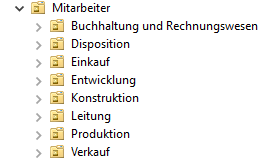
\includegraphics{figures/image1.png}
  \caption{Gliederung der OUs im Active Directory}
  \label{figure:adstructure}
\end{figure}

Die Aufteilung in Standorte ist nicht erforderlich, da die Firma Mikado
nur den Hauptsitz in Köln besitzt.

\chapter{Installation}

Die Installation der Testumgebung wird in einem Hypervisor auf einer
Physikalischen Maschine getestet, da diese Anwendungen im Testbetrieb keine
großen Anforderungen haben. Das Basis Betriebssystem ist ein Hypervisor Server,
welcher von Microsoft kostenlos zur Verf\"ugung gestellt wird. Auf diesem können
unterschiedliche virtuelle Maschinen angelegt werden, welche Ressourcen des
Hostsystems verwenden werden.

\section{Windows Server 2016}\label{windows-server-2016}

F\"ur die Installation des Windows Server 2016 Datacenter wird in dem Hypervisor
zunächst eine leere virtuelle Maschine angelegt. Diese kann anschlie\ss{}end
mit dem Image f\"ur Windows Server 2016 installiert werden. Bei der Installation
des Servers wird eine grafische Benutzeroberfläche verwendet, da auch
unerfahrene Informationstechniker diese bedienen sollen. Innerhalb der
Testumgebung sollen die virtuellen Maschinen eine Festplattengröße von 75GB und
einer Arbeitsspeicher Größe von sechs GB nicht \"uberschreiten. Die virtuellen
Maschinen können im Falle eines Übergangs in den Produktivbetrieb mit weiteren
Ressourcen ausgestattet werden. Nach der erfolgreichen Installation und
Neustart des Servers, muss erstmalig ein Administrator Kennwort festgelegt
werden. Dieses muss folgende Anforderungen besitzen:

\begin{outline}
  \1 Sonderzeichen
  \1 Großbuchstaben
  \1 Zahlen
  \1 Kleinbuchstaben
\end{outline}

Nachdem die Basis Installation nun erfolgt ist, muss der Windows Server
2016 f\"ur die Rolle als Domain Controller vorbereitet werden. Hierzu wird
zunächst eine statische IP Adresse vergeben, da innerhalb der Domäne ein
separater DHCP Server auf einem Windows Server 2012R2 im späteren
Verlauf installiert wird. Desweiteren muss der Rechnername angepasst
werden, da Windows während der Installationsroutine einen f\"ur den Server
festgelegten Namen vordefiniert. Um im Nachhinein die Unterscheidung der
Server zu verbessern, muss hier ein eindeutiger und aussagekräftiger
Name verwendet werden. Der Server muss anschließend neugestartet werden.

\section{Active Directory}\label{active-directory}

Um eine Rolle auf einem Windows Server installieren zu können, muss diese \"uber
den Server-Manager hinzugef\"ugt werden. Über den Punkt Verwalten
\hyp{}\textgreater{} Rollen und Funktionen hinzuf\"ugen, können dem Server neue
Rollen zugewiesen werden. Rollen oder Funktionen können entweder auf einer
virtuellen Festplatte oder aber innerhalb des Computers installiert werden. Der
Server zeigt eine Auflistung aller Rollen und Funktionen an. Sobald eine Rolle
ausgewählt wurde, weist der Server auf weitere Funktionen hin, die benötigt
werden, damit diese ausgewählte Rolle verwendet werden kann.

Damit die Rolle \enquote{Active Directory-Domänendienste} installiert werden
kann, bedarf es folgende weitere Funktionen:

\begin{figure}[H]
  \centering
  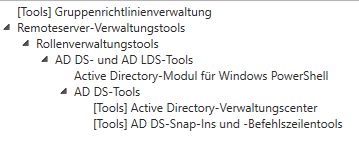
\includegraphics{figures/image2.png}
  \caption{Rollen- und Funktionsverwaltung}
  \label{figure:functions}
\end{figure}

Mit der Schaltfläche \enquote{Features hinzuf\"ugen}, werden anschließend
Funktionen f\"ur die Installationsroutine zugef\"ugt. Nach klicken auf
\enquote{weiter} wird die Meldung ausgegeben, dass der AD-Domänendienst einen
DNS Server innerhalb des Netzwerks benötigt. Sofern dieser nicht vorhanden
sein, wird er auf der gleichen Maschine zusätzlich installiert. Der DNS Server
wird benötigt da dieser f\"ur die Auflösung der Rechnernamen und Druckernamen
zuständig ist. Weitere Erläuterungen hierzu kann im DNS Kapitel entnommen
werden. Abschließend wird eine Übersicht der Installationsroutine angezeigt,
welche mit \enquote{Installieren} bestätigt werden kann.

\section{DNS-Dienst}\label{dns-dienst}

Bereits während der Installation des Domain Controllers, stellt Windows
sicher, ob ein DNS Server installiert werden soll. Jeder DC sollte in der
Regel auch ein DNS Server sein, damit neue Einträge unmittelbar direkt
\"ubertragen werden können und der DNS Dienst immer den aktuellsten Stand
der Umgebung kennt.

\section{DHCP-Dienst}\label{dhcp-dienst}

Die Installation des DHCP Dienstes, kann \"uber den Server-Manager unter
dem Punkt Verwalten \textgreater{} Rollen und Funktionen hinzuf\"ugen
ausgewählt werden. Wie auch bei der Installation des Active Directorys,
zeigt auch hier die Installationsroutine weitere Tools an, die f\"ur die
Verwendung des DHCP Servers empfohlen werden. Diese können \"uber den
Punkt \enquote{Funktionen hinzuf\"ugen} ausgewählt werden. Nach Bestätigung auf
weiter, zeigt die Installationsroutine Informationen \"uber das DHCP an.
Zusätzlich erhält der Benutzer Hinweise das beispielsweise der aktuelle
Server auf dem der DHCP Server installiert werden soll eine statische IP
Adresse besitzen soll, sowie die Subnetze bereits vorher geplant werden
sollen. Nach erneutem Bestätigen auf Weiter, zeigt die
Installationsroutine die Übersicht der Installation an. Hierbei kann
ebenfalls ausgewählt werden, ob der Server selbständig Neustarts
durchf\"uhren soll. Da es sich hierbei aktuell um eine Testumgebung
handelt, kann dieses Kontrollkästchen aktiviert werden. Zum Schluss muss
die Installation mit \enquote{installieren} bestätigt werden. Der Server
beginnt nun mit der Installation des DHCP Servers.

Nachdem der Server neugestartet wurde, ist der DHCP Server aktiv und
muss abschließend noch Konfiguriert werden.

\section{Datei-Dienst}\label{datei-dienst}

Der Dateidienst, spielt gerade in größeren Unternehmen eine wichtige
Rolle, da viele Benutzer Dateien mit anderen Benutzern teilen oder zur
Verf\"ugung stellen wollen. Hierzu kann der von Windows eigene Dateidienst
verwendet werden, da dieser mit Hilfe des Distributed File System und
deren Verwaltungsoberfläche eine einfache Administration möglich ist.

Um den Windows Dateidienst verwenden zu können, muss dieser zunächst
\"uber den Server-Manager hinzugef\"ugt werden. Die Firma Mikado braucht in
erster Linie die Rolle als DFS-Namespace. Damit die Verwaltung des
Dateidienstes dem Administrator vereinfacht wird, sollte zusätzlich zu
dem DFS-Namespace auch der Ressourcen-Manager installiert wird. Dies ist
ein gesondertes Tool und wird nicht automatisch während der
Installationsroutine mit installiert. Der Ressourcen Manager kann jedoch
auch Problemlos nachträglich installiert werden.

Die Installation ist nun abgeschlossen und der Dateidienst, sowie die
Freigaben können konfiguriert werden.

\chapter{Umsetzen der Anforderungen}\label{umsetzen-der-anforderungen}

\section{Einrichtung DHCP Dienst}\label{einrichtung-dhcp-dienst}

Bereits nach der Installation, zeigt der Server Manager an, dass weitere
Konfigurationsschritte f\"ur den DHCP Server notwendig sind. So muss
beispielsweise der DHCP Server innerhalb der Domäne autorisiert werden,
damit die Clients eine entsprechende IP Adresse abrufen können.
Zusätzlich muss das DHCP verschiedene Sicherheitsgruppen anlegen, die
der DHCP Server benötigt. Nach klicken auf \enquote{weiter} werden
Anmeldeinformationen f\"ur die Domäne abgefragt. Hier muss ein Domänen
Administrator eingetragen sein, da nur dieser entsprechende
Autorisierungen des DHCP Servers durchf\"uhren darf. Windows f\"ullt diesen,
da der DHCP Server auf der gleichen Virtuellen Maschine wie der
Domaincontroller installiert ist, standardmäßig mit dem Administrator
aus, da dieser bereits während der Installationsroutine als Domänen
Administrator hinzugef\"ugt wurde. Der Nutzer hat die Möglichkeit,
alternative Anmeldeinformationen anzugeben. Die Autorisierung des DHCP
Servers ist nötigt, falls mehrere DHCP Server innerhalb einer Domäne
arbeiten, da andernfalls es Konflikte zwischen diesen bei der Vergabe
der IP Adressen geben könnte.

Mit klicken auf \enquote{Commit ausf\"uhren} wird die Autorisierung, sowie das
Anlegen der entsprechenden Sicherheitsgruppen im Active Directory
durchgef\"uhrt.

Im Anschluss erhält der Administrator eine Zusammenfassung der
Konfiguration, ob die Konfiguration durchgelaufen ist.

Die Grundkonfiguration des DHCP Server ist abgeschlossen. Als nächsten
Schritten m\"ussen nun innerhalb des DHCP Servers Bereiche definiert
werden. Hierzu muss zunächst unter Tools \textgreater{} DHCP die
Verwaltungskonsole des DHCP aufgerufen werden, da nur in dieser Bereiche
und Konfigurationen durchgef\"uhrt werden können.

Um einen Bereich zu konfigurieren, muss zunächst im DHCP Verwaltungstool
der DHCP Server ausgewählt werden. Anschließend gibt es die Auswahl
zwischen IPv4 oder IPv6. Die Firma Mikado verwendet IPv4, weshalb hier
der Bereich auf IPv4 beschränkt werden kann. Mit Rechtsklick auf IPv4
öffnet sich ein Untermen\"u, wo \enquote{neuer Bereich} ausgewählt wird. Es
öffnet sich ein Bereitstellungs-assistent, welcher den Administrator
durch die Konfiguration leitet. Mit klicken auf \enquote{weiter}, muss zunächst
ein Name f\"ur den Bereich und eine Beschreibung festgelegt werden. Sobald
diese definiert wurde, muss die Start und End IP Adresse definiert
werden, sowie die Subnetzlänge.

Sollte ein IP Adressen Netzwerk viele IP Adressen beinhalten, so schlägt
der Assistent vor, die IP Adressen in Bereichsgruppen aufzuteilen.

Nach bestätigen der IP Adressen, wird abgefragt, ob IP Adressen
ausgenommen werden sollen. Beispielsweise bei Servern oder Applikationen
die immer die gleiche IP Adresse benötigen. Sollten hier keine Ausnahmen
definiert werden m\"ussen, wird anschließend die Lease Time abgefragt. Die
Lease Time bestimmt, wie lange eine IP Adresse f\"ur einen Client g\"ultig
sein darf. Sobald die Lease Time abläuft, f\"ur der Client erneut eine
DHCP Anfrage durch, um erneut die IP Adresse f\"ur sich zu reservieren. Da
es sich bei der Firma Mikado um festdefinierte PCs handelt, empfiehlt es
sich hier die Lease Time auf den Standardwert von 8 Tage belassen.
Sollte beispielsweise die Firma Mikado eine WLAN Infrastruktur, f\"ur
Kunden anbieten, so sollte die Lease Time f\"ur diesen Bereich auf wenige
Stunden herabgesetzt werden.

Eine kurze Lease Time sollte ebenfalls verwendet werden, wenn der DHCP
Server nur einen sehr beschränkten Raum f\"ur IP Adressen besitzt. Sollte
der DHCP Server keine IP Adressen mehr vergeben können, weil
beispielsweise alle vergeben sind, so können keine neuen Geräte mit der
Infrastruktur kommunizieren.

Im nächsten Schritt wird abgefragt, ob die DHCP Optionen aktiviert
werden sollen. Diese definieren, das Standardgateway, den DNS Server,
sowie den WIN Server f\"ur diesen Bereich, welche in der DHCP Abfrage dem
Client zugeschickt wird.

Sobald das Standardgateway abgefragt wurde, werden nachträglich noch die
Einstellungen f\"ur die Domäne sowie den DNS Server und den WinSServer
abgefragt. Abschließend muss entschieden werden, ob dieser Bereich
bereits aktiviert wird oder nachträglich aktiviert werden muss. Sobald
dies bestätigt wurde ist der Bereich fertig konfiguriert.

Diese Einstellung muss nun f\"ur jede Abteilung, sowie f\"ur die Server IP
Range definiert werden.

Bei der Server IP Range ist besonders, dass hier entsprechend die Server
eine Manuelle IP Adressen erhalten, bzw. aus der Adressvergabe des DHCP
Server ausgenommen werden. Die Administrationsrechner erhalten ebenfalls
eine fest zugewiesene IP Adresse und sind in dem gleichen IP Bereich wie
die Server.

Der Aufbau des DHCP Bereiche sieht nun wie folgt aus:

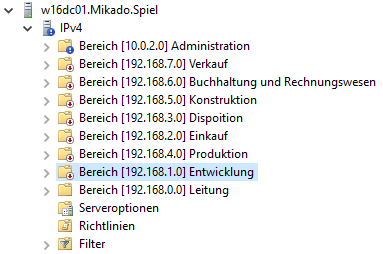
\includegraphics[width=3.98819in,height=2.65139in]{figures/image3.png}

Bereiche, welche deaktiviert sind erhalten an dem Ordnersymbol einen
kleinen roten Pfeil nach unten. Besondere Bereiche oder Bereiche, welche
eine Ausnahme oder eine Aktion erfordern, haben ein weißes
Ausrufezeichen. Aktivierte Bereiche, wie zum Beispiel der Bereich
Leitung erhält keine besonderen Symbole.

Bei dem Anlegen der einzelnen Bereiche wird ebenfalls festgelegt, das
bei neuen Lease Abrufen der Clients, diese automatisch als DNS Einträge
(A-Einträge) festgelegt werden. Dies kann jedoch deaktiviert werden. Um
einen Bereich zu verändern, kann mit einem Rechtsklick die Eigenschaften
wie IP Adressbereich etc. abgeändert werden. Ebenfalls kann hier unter
dem Reiter DNS auch ein DHCP Namensschutz eingerichtet werden. Dies
sorgt daf\"ur, das bereits vorhandene DNS Einträge \"uberschrieben werden
können.

Innerhalb eines Bereiches können Reservierungen f\"ur beispielsweise
Drucker festgelegt werden. Hierzu muss ein entsprechender Bereich
aufgeklappt und anschließend mit Rechtsklick auf Reservierungen die
Reservierung hinzugef\"ugt werden.

Da innerhalb einer Domäne immer ein DHCP Server erreichbar sein sollte,
sollte unter den Eigenschaften des IPv4 ein Sekundärer DHCP Server
eingetragen werden. Dieser \"ubernimmt die Aufgaben und Bereiche, falls
der Primäre DHCP Server nicht mehr antwortet.

Der DHCP Server ist nun vollständig Konfiguriert und kann nun verwendet
werden.

\subsection{Test des Failovers}\label{test-des-failovers}

Um den Test des DHCP Failovers \"uberpr\"ufen zu können, wurde zunächst der
Windows 7 Client, welcher innerhalb des Netzwerks ist gestartet und
anschließend die Eingabeaufforderung gestartet, zudem wurden beide DC
mit entsprechender DHCP Rolle gestartet.

Innerhalb der Eingabeaufforderung, wird nun folgender Befehl eingegeben
damit die aktuelle IP Konfiguration ausgegeben wird:

Ip config /all

Die Eingabeaufforderung, zeigt folgendes Ergebnis:

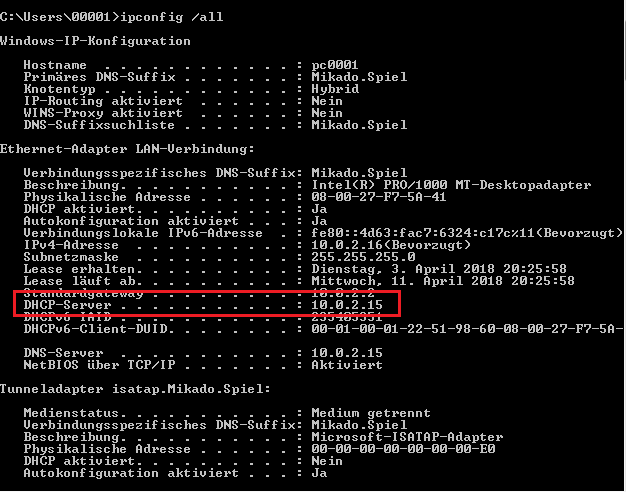
\includegraphics[width=4.10417in,height=3.22561in]{figures/image4.png}

Der Primäre DHCP Server 10.0.2.15 hat dem Client die IP Adresse
10.0.2.16 zugewiesen. Eine IP aus einem nicht reservierten Bereich. Um
den Gegentest durchf\"uhren zu können, wird nun der DHCP-Dienst auf dem
Primären DHCP abgeschaltet und der Client neugestartet. Nach dem
Neustart des Clients, wurde erneut der oben stehende Befehl abgesetzt.
Das Ergebnis sieht danach wie folgt aus:

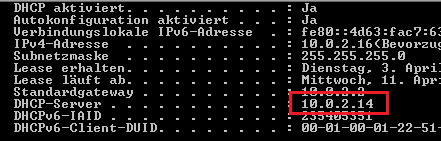
\includegraphics[width=4.59318in,height=1.46857in]{figures/image5.png}

Der Client halt selbständig \"uber den DHCP Broadcast festgestellt, dass
der Primäre Server nicht erreichbar ist und vom Sekundären Server die IP
Adresse, sowie die Leasetime erhalten. Der Sekundäre Server hat somit
die Aufgaben des Primären DHCP Servers \"ubernommen.

\section{Einrichtung DNS Dienst}\label{einrichtung-dns-dienst}

Bereits während der Installation des Active Directory Domänendienst wird
der DNS Dienst angelegt und bereits vorkonfiguriert. Er ist so
eingestellt, dass dieser automatisch aktualisiert wird. Zusätzlich zu
den automatischen Aktualisierungen, können manuelle Einträge als Host A
Eintrag hinzugef\"ugt werden. Diese Einträge können \"uber den DNS-Manager
verwaltet werden. Es gibt zwei Arten der DNS Einträge:

\begin{itemize}
\item
  Host A
\item
  Host AAAA
\end{itemize}

Host A definiert eine IPv4 Adresse und Host AAAA definiert eine IPv6
Adresse. Wenn ein DNS Eintrag manuell eingetragen wird, so muss der FQDN
des Servers/Rechners und deren IP Adresse angegeben werden.

Jede Domäne sollte einen DNS Server haben. Gibt es innerhalb einer
Domäne unter Domänen, so muss dem DNS Server der obergeordneten Domäne
dies mitteilen, damit dieser den DNS Server kennt. DNS Server arbeiten
in der Regel nach dem Prinzip, wissen wo etwas zu finden ist. Sollte der
DNS Server beispielsweise keinen Eintrag in der eigenen \enquote{Datenbank}
finden, so pr\"uft er hier die obergeordnete DNS Struktur, ob ihm dieser
Name bekannt ist. DNS Server haben mehrere Zonen, eine Primäre und eine
Sekundäre Zone. Eine Sekundäre Zone wird meist dann verwendet, wenn eine
Domäne auf eine andere Domäne Zugreifen muss. Die Sekundäre Zone
erstellt eine Kopie dieser und legt sie auf den Server ab.

\section{Dateidienst/Freigaben
einrichten}\label{dateidienstfreigaben-einrichten}

Das Anlegen von neuen Freigaben ist Assistentengesteuert, damit hier die
Anpassungen alle auf einmal durchgef\"uhrt werden können. Um eine Freigabe
hinzuf\"ugen zu können, muss zunächst im Server Manager \textgreater{}
Datei- und Speicherdienste \textgreater{} Freigaben unter Aufgaben eine
neue Freigabe ausgewählt werden:

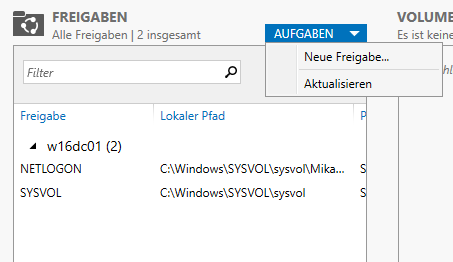
\includegraphics[width=4.71875in,height=2.72917in]{figures/image6.png}

Zum aktuellen Zeitpunkt, besitzt der Server zwei Freigaben. Diese wurden
während der Installation des ActiveDirectorys angelegt. NetLogon soll
dabei f\"ur Anmeldeskripte zur Verf\"ugung stehen.

Sobald auf neue Freigabe geklickt wurde, öffnet sich der Assistent f\"ur
die Freigabe, in dem ein Profil aus folgenden ausgewählt werden muss:

\begin{itemize}
\item
  SMB-Freigabe -- Schnell
\item
  SMB-Freigabe -- Erweitert
\item
  SMB-Freigabe - Anwendungen
\item
  NFS-Freigabe - Schnell
\item
  NFS-Freigabe -- Erweitert
\end{itemize}

Der Unterschied zwischen schnell und erweitert ist in diesem Fall nur
wie viele Informationen während des Assistenten abgefragt werden sollen.
Gleichgestellt wie einfach oder Benutzerdefiniert. Eine SMB Freigabe f\"ur
Anwendungen, soll eine Freigabe f\"ur Hyper-V Manager oder Datenbanken
darstellen.

Der Assistent gibt zu jedem Profil auf der rechten Seite eine kurze
Beschreibung mit, um was es sich bei diesem Profil handelt. F\"ur die
Firma Mikado m\"ussen mehrere SMB Freigaben angelegt werden, weshalb hier
SMB-Freigabe -- Erweitert ausgewählt wird.

Im nächsten Schritt wird nun der Server ausgewählt, auf dem die Freigabe
durchgef\"uhrt werden soll, sowie der Speicherort. Da innerhalb der
Testumgebung zwei DC Servers vorhanden sein werden, kann dies auf dem
Master DC hinterlegt werden. Ein Praktischer Anwendungsfall wäre hier
beispielsweise die Speicherung der Daten auf einem separaten Datei
Server, da auf diesen entsprechende Sicherungen durchgef\"uhrt werden
können.

Als nächstes wird der Freigabename abgefragt, welcher hier verwendet
werden soll. Hier könnte man nun beispielsweise Abteilungsordner
anlegen, welche den Nutzer bei jeder Anmeldung zugewiesen werden, damit
jeder Mitarbeiter auch eine Ablage f\"ur die Abteilung besitzt.

Der Server zeigt nach der Eingabe des Namens unmittelbar den Lokalen,
wie auch den Remotepfad zu dieser Freigabe an:

Lokaler Pfad zur Freigabe:

C:\textbackslash{}Shares\textbackslash{}Leitung

Remote Pfad zur Freigabe:

\textbackslash{}\textbackslash{}w16dc01\textbackslash{}Leitung

Nachdem der Freigabename definiert wurde, werden weitere \enquote{andere
Einstellungen} abgefragt. Diese können f\"ur die Abteilungsfreigabeordner
auf dem Standard belassen werden. Im späteren Verlauf werden noch zwei
Ordner \enquote{Profiles\$} und \enquote{Home\$} angelegt. Bei diesen beiden Freigaben
handelt es sich um die Servergespeicherten Profile. Dabei ist hier die
Besonderheit, das bei dem Punkt \enquote{andere Einstellungen} das
Zwischenspeichern der Freigabe zulassen deaktiviert ist, sowie das \$ am
Ende des Freigabenamens vorhanden ist. Nur mit diesem \$ Zeichen, wird
diese Freigabe nicht f\"ur die Benutzer sichtbar sein.

Damit nicht alle Nutzer Zugriff auf dieses Laufwerk erhalten können,
werden entsprechende Berechtigungen definiert. Innerhalb des
ActiveDirectory, werden Sicherheitsgruppen f\"ur jede Abteilung erstellt,
worin die Benutzer der Abteilung Mitglieder sind.

In diesem Beispiel wäre das die Sicherheitsgruppe: LGs-Leitung

Diese Gruppe soll Lese und Schreibberechtigung auf dieser Freigabe
besitzen, dazu muss unter Berechtigungen anpassen \textgreater{}
hinzuf\"ugen die Sicherheitsgruppe ausgewählt werden. Innerhalb dieses
Fensters, kann die Berechtigung festgelegt werden, die diese Gruppe
erhält. Da in diesem Fall diese Gruppe Schreib und Leseberechtigung auf
diese Freigabe erhalten sollen, wird folgende Berechtigung festgelegt:

\begin{itemize}
\item
  Lesen, ausf\"uhren
\item
  Ordnerinhalt auflisten
\item
  Lesen
\item
  Schreiben
\end{itemize}

Ändern, sowie Vollzugriff erhalten die Benutzer in diesem Falle nicht.
Nach bestätigen auf \enquote{weiter}, wird diese zuvor hinzugef\"ugte Gruppe den
Berechtigungen hinzugef\"ugt. Im nächsten Schritt, wird die
Ordnerverwaltungseigenschaft f\"ur den Verwendungszweck des Freigegeben
Ordners festgelegt. Dies wird wie eine Klassifizierungsregel innerhalb
der Datenverwaltungsrichtlinie festgelegt.

Da es sich bei der Freigabe des Abteilungslaufwerks um eine
Gruppenfreigabe (Benutzer sollen die Möglichkeit haben Daten
untereinander austauschen zu können) handelt, muss dieses entsprechend
ausgewählt werden. Auch hier gibt es wieder die Besonderheit, bei den
Profiles und Home Freigaben. Da es sich bei diesen beiden um Ordner
handeln, die in der Regel nur von einem einzelnen Benutzer verwendet
werden, muss hier die Benutzerdateien ausgewählt werden.

Zum Schluss des Assistenten, kann ein Speicherkontingent festgelegt
werden. Hiermit wird der Speicherbereich limitiert, den der Benutzer zur
Verf\"ugung gestellt bekommt. F\"ur die Abteilungslaufwerke ist dies nicht
erforderlich. Wichtig ist dies in Bezug auf die Servergespeicherten
Profile, sowie umgeleitete Ordner. Hierbei soll der Anwender nur eine
maximale Menge von 200MB ablegen können, damit An- oder Abmeldungen
nicht lange dauern. Benutzer sollen in der Regel Daten, die sie während
der Arbeit brauchen auf dem Abteilungslaufwerk ablegen.

Abschließend erhält der Administrator eine Übersicht \"uber die
Freigabeeigenschaften. Sobald nun auf \enquote{erstellen} geklickt wird, wird
der Freigabe Ordner auf dem Server mit den entsprechenden Berechtigungen
angelegt. Das Ergebnis sollte wie folgt aussehen:

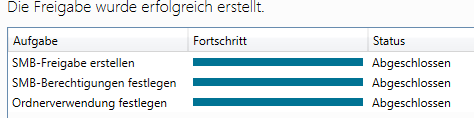
\includegraphics[width=4.9375in,height=1.22917in]{figures/image7.png}

Die Eigenschaften, welche zuvor festgelegt wurden, können nach
abschließen des Assistenten weiterhin bearbeitet und angepasst werden.

Damit Servergespeicherte Profile innerhalb einer Freigabe abgelegt
werden können, muss zunächst wie oben beschrieben jeweils eine Freigabe
f\"ur \enquote{profiles\$} und eines f\"ur \enquote{home\$} angelegt werden.

Hier sollte die Berechtigung auf eine bestimmte Benutzergruppe limitiert
werden. Sinnvoll erscheint es hier eine Sicherheitsgruppe \"uber das AD
anzulegen und diese entsprechend Berechtigung darauf zu gewähren. Die
Berechtigungen auf diese Ordner sollten wie folgt aussehen:

Ordner auflisten/Daten lesen, Attribute lesen, Ordner erstellen/Daten
anhängen

Nur so kann ein Nutzer beim Anmelden ein Benutzerprofil innerhalb dieses
Ordners anlegen und verwalten. Der Nutzer erhält auch nur auf diesen
Ordner die Berechtigungen. Andere Ordner kann der Nutzer nicht sehen
oder verändern.

\subsection{Ressourcen-Manager}\label{ressourcen-manager}

Über den Ressourcen Manager des Dateidienstes, hat der Administrator die
Möglichkeit, verschiedene Kontingente zuzuweisen oder angepasste
Kontingente zu erstellen. Bei einer Überschreitung einer solchen
Kontingentsverletzung, können verschiedene Aktionen durchgef\"uhrt werden.
Beispielsweise kann dem Benutzer eine Systemerzeugte Meldung angezeigt
oder eine Email an den Administrator oder dem Benutzer versendet werden.
Vorausgesetzt es gibt ein Mailserver innerhalb der Umgebung, welcher als
SMTP Server dient. Zusätzlich kann er verschiedene Dateitypen f\"ur das
Speichern auf gewissen Laufwerken verbieten. So kann hier festgelegt
werden, das beispielsweise keine Excel Makros mit *.xlsm Endung auf
einem Laufwerk abgelegt werden kann. Der Ressourcen Manager kann
zusätzlich zu diesen Funktionen auch Logs erzeugen, sowie
Klassifizierungen der Inhalte durchf\"uhren. Hierzu kann entsprechend ein
Zeitplan festgelegt werden, indem das System diese Ordner \"uberpr\"uft.

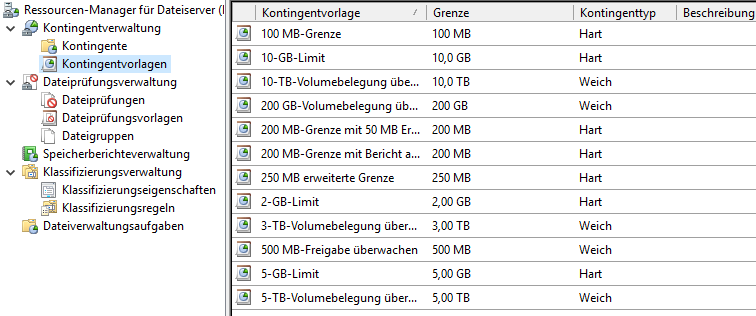
\includegraphics[width=6.3in,height=2.63333in]{figures/image8.png}

\section{Active Directory
Domänendienst}\label{active-directory-domuxe4nendienst}

Nachdem die Grundinstallation abgeschlossen wurde, kann mit der
eigentlichen Konfiguration begonnen werden. Bereits nach der Basis
Installation, makelt der Windows Server \enquote{Konfiguration erforderlich} an
und zeigt einen Link um den Server zum DomainController (DC)
heraufzustufen. Anschließend muss die Art des Domänencontrollers
festgelegt werden. Da es sich hierbei um eine neue Gesamtstruktur mit
neuem DC handelt, muss hier \enquote{Neue Gesamtstruktur hinzuf\"ugen} ausgewählt
werden. Der DC benötigt nun die Stammdomäne, welche \enquote{Mikado.Spiel}
lautet. Dies kann der Fully Qualified Domain Name sein, muss mindestens
jedoch eine Second-Level-Domain sein. Anschließend muss mit weiter
bestätigt werden.

Im nachfolgenden Dialog können Domänencontrolleroptionen eingestellt
werden. Dabei muss nun f\"ur die Gesamtstrukturfunktionsebene, sowie der
Domänenfunktionsebene der älteste DC definiert werden. Da innerhalb der
Testumgebung sowohl ein DC auf einem Windows Server 2012R2 und einer auf
Windows Server 2016 installiert werden muss, muss hier Windows Server
2012R2 ausgewählt werden. Dies kann nachträglich nicht nach unten
korrigiert werden.

Der Kontrollkästchen bei DNS Server sollte gesetzt werden, da jeder DC
auch DNS Server sein kann. Da es sich hierbei um den ersten DC in der
Gesamtstruktur handelt, muss dieser ebenfalls als Globaler Katalog
definiert werden.

Der Globale Katalog dient f\"ur domänen\"ubergreifende Suchfunktionen f\"ur AD
Objekte. Er speichert ausgewählte Attribute aller Objekte aus allen
Domänen.

Abschließend muss hier ein Wiederherstellungskennwort definiert werden,
welches benötigt wird falls AD-Objekte gelöscht wurden um diese
wiederherzustellen. Das Kennwort muss nach dem booten in den
Verzeichnisdienst Wiederherstellungsmodus eingegeben werden. Ohne dieses
können gelöschte AD-Objekte nicht wiederhergestellt werden.

Windows schlägt anschließend einen NetBIOS --Domänennamen vor, welcher
sich aus dem ersten Bestandteil des FQDNs zusammensetzt. Dieser kann
muss jedoch nicht angepasst werden.

Nach erneutem bestätigen auf \enquote{weiter}, werden die Speicherorte f\"ur die
AD DS Datenbanken, sowie Protokolldateien abgefragt. Diese können
ebenfalls bei Bedarf angepasst werden. Die nächste Seite, zeigt nun eine
Gesamt\"ubersicht der Änderungen an, welche zuvor definiert worden sind.
Ebenfalls kann hieraus ein PowerShell Skript erzeugt werden, welches
ggf. angepasst werden kann.

Abschließend \"uberpr\"uft die Installationsroutine ein letztes Mal, ob alle
Einstellungen und Anforderungen erf\"ullt sind. Dabei werden bereits
einige Warnung angezeigt, welche ignoriert werden können. Sobald die
Installationsroutine mit \enquote{installieren} durchgelaufen ist, wird der
Lokale Administrator des Windows Servers automatisch Mitglied der
Gruppen Organisations-, Schema- und Domänen-Admins und hat somit die
Berechtigung Änderungen und Anpassungen durchf\"uhren zu d\"urfen. Ebenso
wird der DNS Server des Windows Servers innerhalb der IP Konfiguration
hinterlegt. Der Windows Server 2016 wird dabei mehrmals neugestartet und
in die Domäne eingebunden.

\subsection{EDV-Struktur im Active
Directory}\label{edv-struktur-im-active-directory}

Der Aufbau des Active Directory, sollte im Regelfall analog der
Unternehmensstruktur aufgeteilt sein. Innerhalb des ADs werden diese in
Organisationseinheiten aufgeteilt. Letztendlich können solche
Organisationseinheiten auch Standorte wiederspiegeln.
Organisationseinheiten sollen bei den Verwaltungsaufgaben helfen. Jeder
Angelegte Benutzer, welcher keiner Organisationseinheit hinterlegt wurde
wird in den Container \enquote{User} abgelegt. Bei mehreren Hundert Nutzern
wären diese alle in dem User Container enthalten. Dies könnte jedoch
gerade in Bezug auf die Rechte vergabe Probleme verursachen, da
unterschiedliche Nutzer auch unterschiedliche Berechtigungen erhalten.
So könnte man je Organisationseinheit unterschiedliche Berechtigungen
zuweisen ohne jeden Nutzer einzeln verändern zu m\"ussen.

Um neue Organisationseinheiten hinzuf\"ugen zu können, muss auf die Domäne
mit Rechtsklick \textgreater{} Neu \textgreater{} Organisationseinheit
geklickt werden. Anschließend kann ein Name f\"ur diese
Organisationseinheit festgelegt werden, sowie festgelegt werden, ob die
Gruppe gelöscht werden kann. Dies soll das versehentliche Löschen der
Gruppe vorbeugen.

Nachdem alle Organisationseinheiten definiert wurden, sieht die Struktur
nun wie folgt aus:

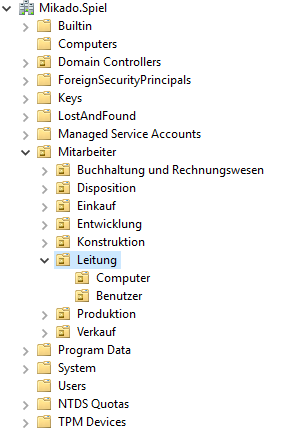
\includegraphics[width=2.98958in,height=4.58333in]{figures/image9.png}

Jede Abteilung hat eine einzelne Organisationseinheit zugewiesen
bekommen. Unter dieser Abtrennung, werden anschließend zwei zusätzliche
Organisationseinheiten angelegt, welche unter Benutzer und Computer
unterschieden wird. Dies hat den Vorteil, dass im Späteren Verlauf die
Gruppenrichtlinien auf einzelne Abteilungen beschränkt werden können. Um
erweiterbare Funktionen einblenden lassen zu können, empfiehlt es sich
unter dem Punkt Ansicht die Erweiterten Features zu aktivieren.

\subsection{Replikation}\label{replikation}

Innerhalb einer Domäne sollte es immer zwei DomainController, sowie zwei
DHCP Server geben. Falls einer der beiden Server ausfällt, können sich
die Nutzer weiterhin Anmelden und erhalten weiterhin eine IP Adresse.

Damit ein zusätzlicher Server in die Domäne integriert werden kann, muss
zunächst eine zusätzliche Maschine bspw. Windows Server 2012 R2
aufgesetzt werden. Nachdem der Server installiert wurde, kann unter
Server-Manager der Domain Controller, wie der erste DC installiert
werden. Domain Controller sind innerhalb einer Domäne gleichberechtigt,
so kann jeder Server die gleichen Aufgaben des anderen \"ubernehmen.

Nachdem die Installation der ActiveDirectory Domänendienste
abgeschlossen wurde, muss dieser zunächst zum DomainController
heraufgestuft werden. Wichtig ist hierbei, dass die Option
Domänencontroller zu einer vorhanden Domäne hinzuf\"ugen ausgewählt sein
muss, damit der DC in die vorhandenen Mikado Domäne zugef\"ugt wird.

Damit die Domäne ausgewählt werden kann, kann Rechts auf \enquote{auswählen}
geklickt werden. Es öffnet sich ein Windows Anmeldefenster, wo die
Anmeldeinformationen von einer Domäne Administrator eingetragen werden
m\"ussen. Wichtig ist hier, dass ein Benutzer eingetragen wird, welcher
die Berechtigung hat, Computer oder Server in die Domäne aufnehmen zu
d\"urfen. Anschließend werden die Domänen Informationen abgefragt und
angezeigt.

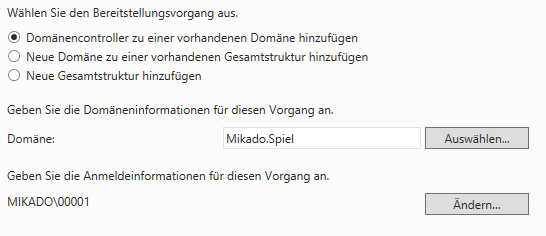
\includegraphics[width=5.6875in,height=2.45833in]{figures/image10.png}

Nachdem die Domäne ausgewählt wurde, kann mit \enquote{weiter} bestätigt
werden. Jeder Domain Controller, sollte gleichzeitig ein DNS Server
beinhalten, sowie ein Globaler Katalog sein, damit hier abfragen
schneller durchgef\"uhrt werden können. Der DNS Server auf dem zweiten
DomainController, kann zudem innerhalb der DHCP Konfiguration als
Sekundärer DNS Server eingetragen werden. Auch hier muss wieder ein
Wiederherstellungskennwort eingetragen werden, welches im Falle vom
versehentlichen Löschen von Ordnern oder AD Strukturen benötigt wird.

Als nächsten Schritt muss die DNS Delegierung, sowie ausgewählt werden,
von welchem DC repliziert werden soll. Da es zum aktuellen Zeitpunkt,
bereits einen DC (w16dc01) gibt, kann dieser nachfolgend ausgewählt und
mit \enquote{weiter} bestätigt werden:

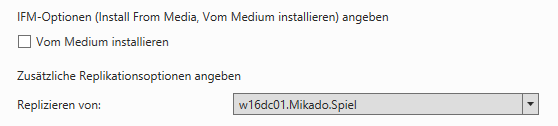
\includegraphics[width=5.8125in,height=1.3125in]{figures/image11.png}

Wie auch bei dem ersten DC, werden auf dem zweiten DC Ordner f\"ur die
Protokollierung, sowie die Datenbank angelegt. Abschließend, gibt die
Installationsroutine die Übersicht f\"ur die anstehenden Änderungen. Mit
klicken auf Installieren, wird der DC Konfiguriert und der Windows
Server einmal neugestartet.

Die Replikation ist nun abgeschlossen. Alle Änderungen, welche fortan
auf dem DC01 durchgef\"uhrt werden, werden innerhalb weniger Sekunden auf
den DC02 repliziert. Sollte eine Replizierung der Daten aussetzen, so
ruft der DC02 automatisch nach einer Stunde die Informationen ab.

Nachdem der Server erneut gestartet wurde, kann die Anmeldung mit dem
Administrator vom DC01 durchgef\"uhrt werden.

\hypertarget{benutzerkonten-erstellen}{%
\subsection{Benutzerkonten
erstellen}\label{benutzerkonten-erstellen}}

Benutzer können \"uber die Active Directory Benutzer und
Computerverwaltungs\"ubersicht manuell hinzugef\"ugt werden. Hierzu kann
innerhalb einer OU mit Rechtsklick \textgreater{}Neu \textgreater{}
Benutzer ein Benutzer hinzugef\"ugt werden. Der Benutzer wird nun direkt
in die richtige OU angelegt.

In dem dann neu eröffneten Fenster muss nun ein Vorname, Nachname und
Benutzername festgelegt werden. Der Benutzername muss innerhalb einer
Domäne eindeutig sein und besteht bei der Firma Mikado als 5 stellige
Personalnummer. Eine Personalnummer darf nie doppelt vergeben werden, da
diese zusätzlich in der Buchhaltung als Referenz f\"ur den Mitarbeiter
verwendet wird. Nachdem diese Informationen eingetragen wurden, muss mit
\enquote{weiter} bestätigt werden. Es folgt die Abfrage nach dem
Benutzerkennwort, womit sich dieser an einem Rechner oder Domäne
anmelden kann. Das Kontrollkästchen bei \enquote{Benutzer muss Kennwort bei der
nächsten Anmeldung ändern} sollte angehakt sein, damit der Anwender ein
eigenes von ihm definierte Kennwort erstellen kann. Hier kann man
beispielsweise nun ein Kennwort verwenden, welches der
Standardrichtlinien entspricht. Als Beispiel wäre hier \enquote{Mikado2018!}
möglich, da es sowohl klein-, Großbuchstaben, sowie Sonderzeichen und
Zahlen enthält.

Nachdem der Anwender sich hiermit an einem Rechner innerhalb der Domäne
anmeldet, wird automatisch die Änderung des Kennworts verlangt. Ohne
dieses ist keine Anmeldung an der Domäne möglich.

Sollte es sich bei dem angelegten Nutzer um einen Service Account
handeln, beispielsweise FTP Zugriff oder sonstiges, empfiehlt es sich
hier, das Kennwort nicht ablaufen zu lassen, sowie das Kontrollhäckchen
bei \enquote{Benutzer muss Kennwort bei der nächsten Anmeldung ändern}
rauszunehmen, da andernfalls die Funktion dieses Service Accounts
eingeschränkt sein könnte.

Zum Schluss wird eine Übersicht \"uber den Nutzer angezeigt.

\hypertarget{gruppenkonten-erstellen}{%
\subsection{Gruppenkonten erstellen}\label{gruppenkonten-erstellen}}

Ein Gruppenkonto, kann entweder in einer Abteilungs OU oder in dem
Container User erstellt werden. Hierzu muss man innerhalb des
gew\"unschten Verzeichnis mit der rechten Maustaste \textgreater{} Neu
\textgreater{} Gruppe die Gruppe hinzuf\"ugen. Es öffnet sich ein neues
Fenster, wo weitere Einstellungen vorgenommen werden können. In der
Regel muss hier zunächst ein Gruppen Namen definiert werden. Dabei
sollte geachtet werden, dass der Gruppenname eindeutig zu der Funktion
der Gruppe ist, da im späteren Verlauf nur der Gruppennamen angezeigt
wird, jedoch nicht deren Funktion. Zusätzlich ist gegebenenfalls
hilfreich anzugeben, f\"ur welche Abteilung dieses Gruppe ist.

Gruppen haben drei Gruppenbereiche und zwei Gruppentypen zur Auswahl.
Die Gruppenbereiche geben an, welche Benutzerkonten und Computerkonten
Mitglied von dieser Gruppe sein d\"urfen und von welcher Domäne. Hierzu
gibt es folgende Erläuterung:

\begin{longtable}[]{@{}lll@{}}
\toprule
Gruppenbereich & Mitgliedschaft & Verwendbarkeit\tabularnewline
\midrule
\endhead
\begin{minipage}[t]{0.30\columnwidth}\raggedright
Lokal (in Domäne)\strut
\end{minipage} & \begin{minipage}[t]{0.30\columnwidth}\raggedright
Benutzer- und Computerkonten beliebiger Domänen,

globale und universelle Gruppen beliebiger Domänen,

lokale Gruppen derselben Domäne\strut
\end{minipage} & \begin{minipage}[t]{0.30\columnwidth}\raggedright
Nur in derselben Domäne\strut
\end{minipage}\tabularnewline
\begin{minipage}[t]{0.30\columnwidth}\raggedright
Global\strut
\end{minipage} & \begin{minipage}[t]{0.30\columnwidth}\raggedright
Benutzer- und Computerkonten derselben Domäne,

globale Gruppen derselben Domäne\strut
\end{minipage} & \begin{minipage}[t]{0.30\columnwidth}\raggedright
In beliebigen Domänen\strut
\end{minipage}\tabularnewline
\begin{minipage}[t]{0.30\columnwidth}\raggedright
Universal\strut
\end{minipage} & \begin{minipage}[t]{0.30\columnwidth}\raggedright
Benutzer- und Computerkonten beliebiger Domänen,

globale und universale Gruppen beliebiger Domänen\strut
\end{minipage} & \begin{minipage}[t]{0.30\columnwidth}\raggedright
In beliebigen Domänen\strut
\end{minipage}\tabularnewline
\bottomrule
\end{longtable}

Die zwei Gruppentypen sind unterteilt in \textbf{Sicherheit} und
\textbf{Verteilung}. \textbf{Sicherheitsgruppen} können
Sicherheitsrichtlinien zugewiesen werden und können somit den Zugriff
auf Ressourcen zulassen oder verweigern. Bei \textbf{Verteilungsgruppen}
wird der Nutzer, welcher Mitglied dieser Gruppe ist in einen Verteiler,
beispielsweise Mailverteiler hinzugef\"ugt. Verteilergruppen erhalten nach
erstellen ebenfalls eine Email Adresse, an denen Benutzer beispielsweise
eine Email schreiben könnten.

Nachdem eine Sicherheitsgruppe erstellt wurde, kann sie nachträglich mit
einem doppelklick auf dieser bearbeitet werden. Unter den Reitern
Mitglieder, können Benutzer hinzugef\"ugt werden. Dieser Änderungen werden
bei Sicherheitsgruppen erst nach erneuter Anmeldung mit dem
Benutzerkonto sichtbar.

Bereits beim Anlegen der einzelnen Organisationseinheiten, hat das
Active Directory automatisch Sicherheitsgruppen mit dem selbigen Namen
angelegt. Alle Benutzer, die in den einzelnen Organisationseinheiten
sind, sind automatisch Mitglied dieser Sicherheitsgruppe.

\hypertarget{computerkonten-erstellen}{%
\subsection{Computerkonten
erstellen}\label{computerkonten-erstellen}}

Computerkonten können Analog wie auch die Benutzerkonten erstellt
werden. Die Computerkonten, sollten auch hier unmittelbar direkt in der
richtigen OU hinterlegt werden, damit Computerrichtlinien exakt
angewandt werden können. Der Computername sollte ebenfalls wie auch der
Benutzername eindeutig sein, damit hier innerhalb der Domäne keine
Konflikte auftreten können. Zusätzlich zu dem Benutzernamen, muss
definiert werden, welcher Nutzergruppe den Computer in die Domäne
integrieren kann. Dies ist in der Regel nicht f\"ur alle Nutzer gestattet.
Wichtig bei der Namensgebung ist auch die Konvention f\"ur den DNS Server,
da unmittelbar nach Anlegen des Computers, dieser ebenfalls dem DNS
bekannt wird. Sobald dieser sich im Netzwerk meldet, wird er \"uber den
DHCP Server in die Zone aufgenommen und hinterlegt.

\hypertarget{skript-zum-anlegen-von-nutzern-computern}{%
\subsection{Skript zum Anlegen von Nutzern,
Computern}\label{skript-zum-anlegen-von-nutzern-computern}}

Anlegen von Nutzern oder Computern und Zuweisung f\"ur deren Richtlinie,
kann entweder manuell durchgef\"uhrt werden oder aber mittels Script~\cite{Microsoft_technet}
ausgef\"uhrt werden. Zusätzlich zu diesem Skript, gibt es ebenfalls noch
das Anmeldeskript, worauf nachträglich im nächsten Kapitel eingegangen
wird.

\$password = „XTi114!`` \textbar{} ConvertTo-SecureString -AsPlainText
-Force

New-ADUser -Name 'Nikolai Luis' -SamAccountName 00003 -UserPrincipalName
00003 -DisplayName 'Nikolai Luis' -GivenName Nikolai -Surname Louis
-Path „OU=Benutzer,OU=Leitung,OU=Mitarbeiter,DC=Mikado,DC=Spiel``
-AccountPassword \$Password -ChangePasswordAtLogon \$True -Enabled
\$True -ProfilePath
\textbackslash{}\textbackslash{}w16dc01\textbackslash{}profiles\$\textbackslash{}00003
-hmdir
\textbackslash{}\textbackslash{}w16dc01\textbackslash{}home\$\textbackslash{}00003

Das oben stehende PowerShell Skript, f\"ugt einen vordefinierten Benutzer
an die angegebene OU und DC ein. Er erhält ein Passwort \enquote{XTi114!}
welches nach der Anmeldung direkt geändert werden muss. Bedingt dadurch
das die PS Eingabe keine Klartext Passwörter verwenden kann, muss dieses
zuvor in einen Sicheren String umgewandelt werden.

\hypertarget{anmeldeskript}{%
\subsection{Anmeldeskript}\label{anmeldeskript}}

Ein AnmeldeSkript wird während der Anmeldung eines Nutzers geladen und
angewendet. In einem solchen, können beispielsweise Netzlaufwerke,
Drucker oder Freigaben eingef\"ugt sein. Es gibt verschiedene
Möglichkeiten, Benutzern ein Anmeldeskript zur Verf\"ugung zu stellen. Der
einfachste Weg, wäre \"uber eine Gruppenrichtlinie das Anmeldeskript zur
Verf\"ugung zu stellen. Es kann jedoch auch unmittelbar direkt an das
Benutzerprofil beigef\"ugt oder an einen Computer zugewiesen werden.

Das Anmeldeskript als solches ist immer in einem Freigegeben Ordner
\enquote{Netlogon} auf einem DC gespeichert, wo der Nutzer hinterlegt ist.
Innerhalb des Benutzerprofil oder Gruppenrichtlinie, wird anschließend
nur der Name des Skripts hinterlegt. Das ActiveDirectory ergänzt
eigenständig den Pfad zu diesem Skript.

Zusätzlich zum Anmelden eines Benutzers, kann ein Skript auch beim
Abmelden, starten oder Herunterfahren des Computers. Es spielt keine
Rolle, wie viele Anmeldeskripte einem Benutzer zugewiesen wurden.
Windows arbeitet alle Skripte nacheinander ab.

Die Anmeldeskripte, werden nach dem Hinterlegen im Netlogon Ordner auf
die anderen DCs repliziert, sodass alle DCs die gleichen Skripte
besitzen.

\hypertarget{servergespeicherte-benutzerprofile}{%
\subsection{Servergespeicherte
Benutzerprofile}\label{servergespeicherte-benutzerprofile}}

Servergespeicherte Benutzerprofile werden immer dann wichtig sein, wenn
sich ein Benutzer an mehreren unterschiedlichen Rechnern anmeldet. Die
Erzeugten und bearbeiteten Daten oder Dokumente, werden beim Abmelden
auf den Server zur\"uckgesichert. Meldet sich ein Benutzer an einem
anderen Rechner wieder an, so werden die Daten bzw. das Profil vom
Server heruntergeladen. Es gibt insgesamt zwei Arten von
Servergespeicherten Profilen. Einmal die Veränderbaren Benutzerprofile,
dabei werden alle Änderungen innerhalb der Sitzung zum Server
zur\"uckgesichert beim Abmeldet. Die andere Art sind verbindliche Profile.
Diese aktualisieren ein bereits vorhandenes Profil mit den Neuerungen,
welche auf dem Server vorhanden sind.

Im Fall der Firma Mikado, werden Veränderbare Benutzerprofile verwendet,
da im späteren Verlauf zusätzlich die Richtlinie angewandt wird, dass
Benutzerprofile nach Abmelden vom Rechner entfernt werden.

Um die Servergespeicherten Profile konfigurieren zu können, muss unter
der Verwaltungskonsole des Active Directorys, die Benutzereigenschaften
aufgerufen werden. Diese Einstellungen können bereits während des
Anlegens oder mittels Anlegeskript erzeugt werden.

Unter dem Reiter \enquote{Profil}, kann unter Profilpfad der Pfad zu der
Freigabe eingetragen werden. Wichtig ist hierbei die Variable
\%username\%. Damit weiß das Active Directory, das diese Stelle durch
den Benutzernamen, in unserem Fall die Personalnummer ersetzt werden
soll. Sobald ein Benutzer sich nun mit seinem Benutzernamen an einem
Domänenrechner anmeldet, wird f\"ur ihn ein entsprechendes Profil
innerhalb des Profiles Ordner angelegt.

Benutzerprofile sind immer Windows Version abhängig. Ein Nutzer, welcher
mit seiner Benutzerkennung an einem Windows XP Client angemeldet war,
kann sich mit diesem Profil nicht an einem Windows 7 Rechner anmelden,
da hier die Struktur der Ordner unterschiedlich ist.

\hypertarget{heimatverzeichnisse}{%
\subsection{Heimatverzeichnisse}\label{heimatverzeichnisse}}

Zusätzlich zu Servergespeicherten Profilen, wird in der Regel auch eine
Umleitung der Ordner Dokumente, Desktop etc. durchgef\"uhrt. Dies hat die
Vorteile, dass eine An- und Abmeldung schneller durchgef\"uhrt werden
kann, als wenn diese Ordner innerhalb des Profils gespeichert werden.
Die entsprechenden Dokumente, sind f\"ur einen Benutzer anschließend \"uber
ein Netzlaufwerk zu erreichen, wo unter anderem auch das Benutzerprofil
abgelegt ist. Wichtig ist dabei, dass diese Ablage von dem Profilserver
separiert ist, da andernfalls ein Benutzer an diese Daten nicht
drankommen könnte, falls der Profilserver nicht erreicht wäre.
Heimatverzeichnisse, bzw. Ordnerumleitung werden nicht in dem
Benutzer-profil/-eigenschaft hinterlegt, sondern innerhalb einer
Gruppenrichtlinie festgelegt. Diese kann anschließend entweder an einen
Nutzer oder aber Computer zugewiesen sein.

Um die Umleitung der Ordner zu aktivieren, muss zunächst die Default
Domain Policy angepasst werden. Hierzu wird unter Tools die
Gruppenrichtlinienverwaltung geöffnet.

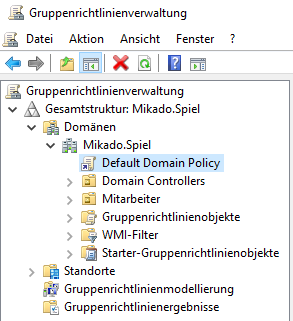
\includegraphics[width=3.05208in,height=3.34375in]{figures/image12.png}

Mit Rechtsklick auf Default Domain Policy, kann diese bearbeitet und
angepasst werden. Es empfiehlt sich hier gegebenenfalls ein zusätzliches
Gruppenrichtlinienobjekt anzulegen. Innerhalb diesem muss um die
Ordnerumleitung verwalten zu können unter Benutzerkonfiguration
\textgreater{} Windows-Einstellungen navigiert werden. Unter dem Punkt
Ordnerumleitung, werden alle Benutzerordner angezeigt:

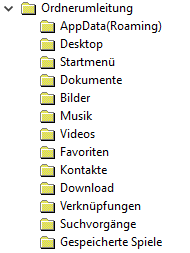
\includegraphics[width=1.97917in,height=2.63542in]{figures/image13.png}

Wichtig hierbei ist, dass die größten Ordner umgeleitet werden, wie
beispielsweise AppData, Desktop, Dokumente, Bilder, Musik etc. Um die
Umleitung zu aktivieren, muss ein Ordner ausgewählt werden und
anschließend \"uber Rechtsklick Eigenschaften bearbeitet werden.

Unter den Eigenschaften, kann nun das Ziel sowie Einstellungen
vorgenommen werden. Unter dem Punkt Ziel muss zunächst als Zielordner:
\enquote{Einen Ordner f\"ur jeden Benutzer im Stammpfad erstellen} ausgewählt
sein. Anschließend wird das Stammverzeichnis unter Angabe des UNC-Pfads
festgelegt. Unmittelbar nach Eingabe des UNC-Pfads, zeigt das Fenster
bereits eine Vorschau des Pfades zu diesem Nutzer an:

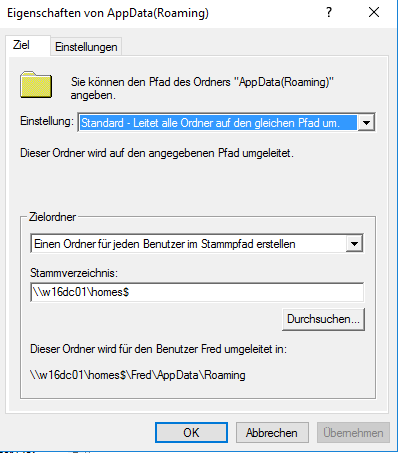
\includegraphics[width=4.14583in,height=4.71875in]{figures/image14.png}

Exemplarisch wurde dies f\"ur die AppDaten des Anwenders durchgef\"uhrt.
Zusätzlich zu diesen Einstellungen, kann festgelegt werden, ob dem
Nutzer exklusive Zugriffsrechte f\"ur Dokumente erteilt werden. Dies kann
ein Nachteil f\"ur den Administrator sein, da dieser im Falle einer
Problemlösung innerhalb des Profils den Besitz \"ubernehmen muss und
anschließend wieder zur\"uckschreiben muss. Sollten dabei Fehler
unterlaufen, so könnte der Benutzer nicht mehr auf diese Daten
zugreifen. Die Einstellung \enquote{Den Inhalt von
\textless{}Ordnername\textgreater{} an den neuen Speicherort
verschieben} sollte aktiviert werden, da durch diesen der Ordner auf
dem Rechner gelöscht und an den zuvor definierten Speicherort verschoben
wird. Sollte diese Option nicht aktiviert sein, so verbleibt eine Kopie
des Ordners auf dem Rechner. Im letzten Abschnitt kann festgelegt
werden, was passieren sollen, falls die Richtlinie entfernt wird.

Zum Abschluss sollten die Einstellungen wie folgt aussehen:

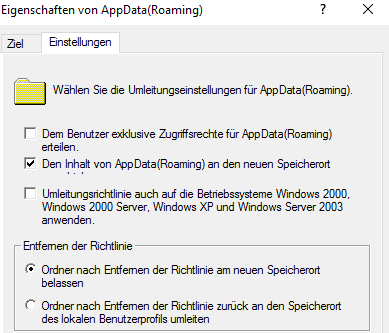
\includegraphics[width=4.05208in,height=3.46875in]{figures/image15.png}

Nach Klicken auf \enquote{ok} wird eine Fehlermeldung ausgegeben, die f\"ur
ältere Betriebssysteme entscheiden ist. Diese kann jedoch bei Verwendung
von Windows 7 oder neuer ignoriert und mit \enquote{Ja} bestätigt werden. Die
zuvor eingestellten Anpassungen, m\"ussen nun f\"ur die restlichen Ordner
ebenfalls durchgef\"uhrt werden, damit die Ordnerumleitung auch auf die
restlichen Aktiviert wird.

Die Ordner Bilder, Musik und Videos, können dem Ordner Dokumente folgen,
so muss f\"ur diese nicht zusätzlich ein Pfad mit angeben werden.

Die Benutzerkonfiguration f\"ur die Ordnerumleitung ist nun abgeschlossen.
Nachträglich m\"ussen noch weitere Computerkonfigurationen vorgenommen
werden, damit auch der Computer f\"ur Servergespeicherte Profile
konfiguriert ist. So m\"ussen beispielsweise Einstellungen vorgenommen
werden, das der Computer auf das Netzwerk wartet, oder aber das die
Sicherheitsgruppe \enquote{Administrator} dem Servergespeichertem Profil
hinzugef\"ugt wird, damit hier bei einer Problemlösung am Benutzerprofil
der Profilbesitzer nicht gewechselt werden muss.

Diese Einstellungen, m\"ussen ebenfalls in der Default Domain Policy, oder
aber in der zuvor erstellten Policy unter dem Punkt
Computerkonfiguration \textgreater{} Richtlinien \textgreater{}
Administrative Vorlagen angepasst werden.

Folgende Punkte m\"ussen hier f\"ur eine erfolgreiche Umleitung der Ordner
eingerichtet werden:

\begin{longtable}[]{@{}l@{}}
\toprule
\endhead
\vtop{\hbox{\strut System \textgreater{} Benutzerprofile \textgreater{}
Sicherheitsgruppe „Administrator`` zu servergespeicherten Profilen
hinzuf\"ugen}\hbox{\strut System \textgreater{} Benutzerprofile
\textgreater{} Zeitlimit f\"ur langsame Netzwerkverbindung f\"ur
Benutzerprofile steuern}\hbox{\strut System \textgreater{} Anmelden
\textgreater{} Beim Neustart des Computers und bei der Anmeldung immer
auf das Netzwerk warten}\hbox{\strut Netzwerk \textgreater{}
Offlinedateien \textgreater{} Alle Offlinedateien vor der Abmeldung
synchronisieren}\hbox{\strut Netzwerk \textgreater{}Offlinedateien
\textgreater{} Untergeordnete Ordner immer offline verf\"ugbar
machen}}\tabularnewline
\bottomrule
\end{longtable}

Nachdem diese Einstellungen innerhalb der Computerkonfiguration
aktiviert wurden, ist die Ordnerumleitung aktiviert und kann verwendet
werden. Sollte hierbei eine Benutzerdefinierte Domain Policy verwendet
worden sein, so muss diese zusätzlich noch f\"ur die einzelne Domäne
hinterlegt werden.

Ein Heimatverzeichnis muss nicht mittels Anmeldeskript angebunden
werden. Dieses kann ebenfalls \"uber eine Gruppenrichtlinie oder innerhalb
des Nutzerprofiles unter Eigenschaften \textgreater{} Profil
\textgreater{} Basisordner verlinkt werden.

\hypertarget{speichervolumen-begrenzung}{%
\subsection{Speichervolumen
Begrenzung}\label{speichervolumen-begrenzung}}

Wie bereits in Kapitel Dateidienst/Freigaben einrichten erläutert, gibt
es verschiedene Möglichkeiten, das Dateilimit innerhalb eines Ordners zu
limitieren. Die Anforderung der Firma Mikado besteht darin, dass ein
Angestellter ein maximales Speichervolumen von 200MB besitzt. Um diese
Kontingentgrenze definieren zu können, muss zunächst innerhalb des
Ressourcen Managers f\"ur Dateiserver, ein neues Kontingent angelegt
werden. Hierzu kann eine bestehende Kontingentgrenze als Vorlage
verwendet werden. Anschließend muss der Kontingentpfad angeben werden.
In diesem Fall:\\
C:\textbackslash{}Shares\textbackslash{}profiles\\
C:\textbackslash{}Shares\textbackslash{}home

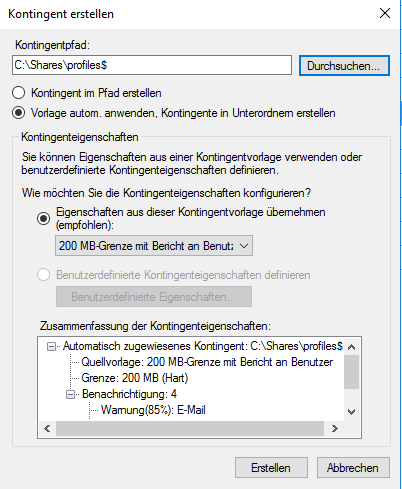
\includegraphics[width=4.1875in,height=5.09375in]{figures/image16.png}

Nachdem der Pfad zu dem Kontingent angelegt wurde, muss die Vorlage
automatisch Anwenden. Kontingente in Unterordern erstellen ausgewählt
werden. Dies bedeutet, dass das Kontingentlimit nur auf die Unterordner
bezogen wird, welche innerhalb dieses Ordners angelegt werden, jedoch
nicht auf den gesamten Ordner. Dies hat den Vorteil, dass jeder Benutzer
ein eigenes Kontingent von 200MB besitzt.

Als Kontingenttyp wird hier hart ausgewählt. Der Unterschied zwischen
harter Kontingent und weicher Kontingent ist der folgende:

Weiche Kontingentgrenze:

\begin{itemize}
\item
  Die Speichergrenze kann \"uberschritten werden, eine Aktion, wie
  beispielsweise Email Versand, Fehler oder Befehl wird ausgef\"uhrt.
  Speichererweiterung um 50MB möglich.
\item
  Dient nur der Überwachung
\end{itemize}

Harte Kontingentgrenze:

\begin{itemize}
\item
  Die Speichergrenze kann nicht \"uberschritten werden
\item
  Limitierung des Speicherplatzes
\end{itemize}

Abschließend sehen die Kontingenteinträge wie folgt aus:

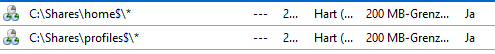
\includegraphics[width=5.15625in,height=0.5625in]{figures/image17.png}

Um eine Weiche Kontingentgrenze zu definieren, muss entsprechend in der
Abbildung xy die Eigenschaft \enquote{Benutzerdefinierte Kontingentgrenze
definieren} ausgewählt sein. Sobald auf Benutzerdefinierte Eigenschaft
geklickt wird, öffnet sich ein neues Fenster, wo die Grenzen, wie
weiche- oder harte Kontingentgrenze, sowie deren Aktion ausgewählt und
definiert werden kann.

\hypertarget{einrichten-von-druckern}{%
\section{Einrichten von Druckern}\label{einrichten-von-druckern}}

Innerhalb einer Domäne kann es einen Druck -- und Dokumentenserver
geben. Dieser stellt den Clients Drucker oder Dokumente zur Verf\"ugung.
Hierbei handelt es sich um eine Rolle, welche innerhalb des
Server-Managers hinzugef\"ugt werden muss.

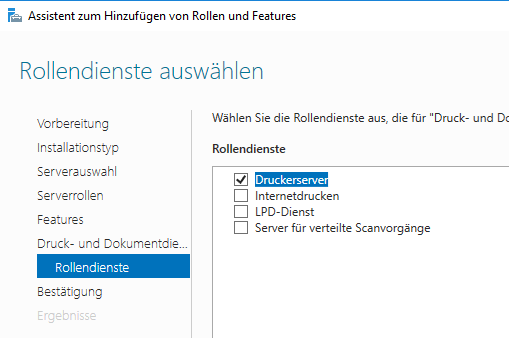
\includegraphics[width=5.30208in,height=3.52083in]{figures/image18.png}

Sollte es innerhalb der Domäne Unix Systeme, wie Ubuntu oder ArchLinux
geben, so sollte hier der Punkt LPD-Dienst aktiviert werden.

Nachdem die Rolle hinzugef\"ugt wurde, kann diese \"uber die Druckverwaltung
administriert werden.

Ein Druckerserver bietet die Möglichkeit, Netzwerkdrucker und deren
Treiber zur Verf\"ugung zu stellen, so muss ein Client, welcher den
Drucker \"uber ein Anmeldeskript zugewiesen bekommt die Installation nicht
manuell anstoßen und Windows muss nicht die Windows Updates f\"ur die
Druckertreiber durchsuchen. Druckertreiberaktualisierungen können so
Zentral gesteuert werden.

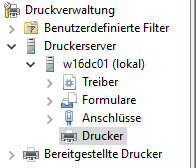
\includegraphics[width=2.04167in,height=1.75in]{figures/image19.png}

Über Rechtsklick, können unter \enquote{Drucker hinzuf\"ugen} weitere Drucker
hinzugef\"ugt werden. Diese können anschließend \"uber die GPO dem Benutzer
zur Verf\"ugung gestellt werden. Der Netzwerkdruckerassistent durchsucht
eigenständig das Netzwerk, nach dem angegeben Druckern.

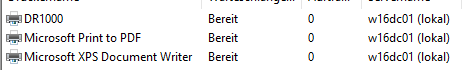
\includegraphics[width=4.84375in,height=0.72917in]{figures/image20.png}

\hypertarget{gruppenrichtlinien}{%
\section{Gruppenrichtlinien}\label{gruppenrichtlinien}}

Gruppenrichtlinien bestehen aus zwei Teilen und sind ein mächtiges
Verwaltungs. Der erste Teil, besteht aus der Computerkonfiguration.
Diese zieht immer auf einem Computer, egal welcher Nutzer angemeldet
ist. Der zweite Teil besteht aus der Benutzerkonfiguration, welche
spezifisch f\"ur die Nutzer definiert werden können. Ein kleines Beispiel
soll dies verdeutlichen:

Die Kennwortrichtlinie ist innerhalb der BenutzerKonfiguration so
eingestellt, dass eine Komplexität von 8 Zeichen benötigt wird. Sobald
ein Nutzer versucht das Kennwort auf dem Rechner anzupassen, kann dieser
jedoch ein Kennwort mit nur einer Länge vergeben, da die
Computerkonfiguration keine Richtlinie f\"ur das Kennwort vorgibt.

Gruppenrichtlinien, werden immer an eine Sicherheitsgruppe gebunden,
welche anschließend einem Benutzer zugewiesen werden kann. Standardmäßig
sind keine Richtlinien oder Einschränkungen festgelegt. Innerhalb einer
Sicherheitsgruppe, können mehrere Gruppenrichtlinien zugewiesen sein.
Wichtig ist hierbei die Verkn\"upfungsreihenfolge der einzelnen GPOs.
Sollte in der ersten Gruppenrichtlinie etwas deaktiviert sein, jedoch in
der zweiten aktiviert, so greift hier die Gruppenrichtlinie, welche an
erster Stelle steht.

Unterschieden wird auch ob eine GPO erzwungen ist. Sollte eine GPO
erzwungen werden, so greift stets die GPO wo diese Einstellung
festgelegt wurde.

\hypertarget{kontorichtlinien}{%
\section{Kontorichtlinien}\label{kontorichtlinien}}

Kontorichtlinien, sind Vorgaben die ein Benutzer erf\"ullen muss. Sie
können beispielsweise die Länge eines Kennworts sein oder andere
ähnliche Einstellungen.

\hypertarget{kennwortrichtlinien}{%
\subsection{Kennwortrichtlinien}\label{kennwortrichtlinien}}

F\"ur die Mikado.Spiel Domäne als Testumgebung sind folgende
Kennwortrichtlinien definiert worden:

\begin{longtable}[]{@{}ll@{}}
\toprule
Eigenschaft & Vorgabe\tabularnewline
\midrule
\endhead
Kennwort erforderlich & Ja\tabularnewline
Länge & 8 Zeichen\tabularnewline
Alter & 50 Tage\tabularnewline
Wiederbenutzbar & Nach 12 Kennwörtern\tabularnewline
\bottomrule
\end{longtable}

Um diese Kennwortrichtlinie festlegen zu können, muss entweder innerhalb
der Standard Gruppenrichtlinie(Default Global Policy) oder in einer
neuen zuvor definierten Gruppenrichtlinie folgende Werte unter
Computerkonfiguration \textgreater{} Windows-Einstellungen
\textgreater{} Sicherheitseinstellungen \textgreater{} Kontorichtlinien
geändert werden:\\
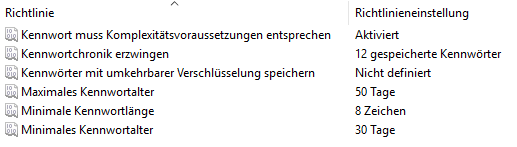
\includegraphics[width=5.38542in,height=1.53125in]{figures/image21.png}

Nun ist die Kontorichtlinie f\"ur die Sicherheitsgruppe aktiv, f\"ur die
diese Richtlinie zugewiesen ist.

\hypertarget{anmelderichtlinien}{%
\subsection{Anmelderichtlinien}\label{anmelderichtlinien}}

Zusätzlich zu Kennwortrichtlinien, hat die Firma Mikado die Richtlinie,
das sich die Mitarbeiter nur während der Arbeitszeit von Montag bis
Freitag zwischen 08:00Uhr bis 18:00 Uhr im Netzwerk anmelden d\"urfen.
Hierzu ist seitens des Domaincontroller zu Limitieren, das eine
Anmeldung auch außerhalb dieser Zeiten durchgef\"uhrt werden kann. Diese
Einstellung, wird nicht in einer Gruppenrichtlinie definiert, sondern
f\"ur jeden Benutzer innerhalb der Active Directory-Benutzer und Computer
verwaltungsoberfläche festgelegt.

Unter dem Reiter Konto \textgreater{} Anmeldezeiten, können die
Anmeldezeiten durch auswählen festgelegt werden.

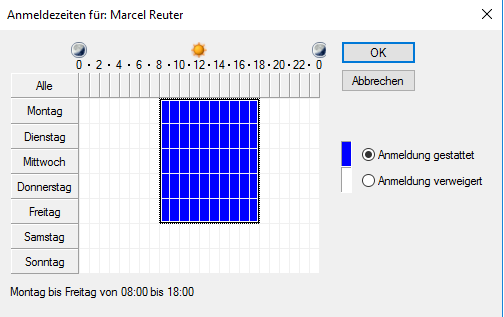
\includegraphics[width=5.25in,height=3.30208in]{figures/image22.png}

Sollte ein Benutzer versuchen außerhalb dieser Zeiten eine Anmeldung
durchzuf\"uhren, so erhält er folgende Meldung:

Das Konto sieht es nicht vor, dass Sie sich zu dieser Zeit anmelden.
Wiederholen Sie diesen Vorgang später.

\hypertarget{administrator-account-umbenennen}{%
\subsection{Administrator Account
umbenennen}\label{administrator-account-umbenennen}}

Die Anpassung des Lokalen Administrator eines Clients, kann ebenfalls
\"uber eine Gruppenrichtlinie festgehalten und verändert werden. Hierzu
muss unter Benutzerkonfiguration \textgreater{} Einstellungen
\textgreater{} Systemsteuerungseinstellungen \textgreater{} Lokale
Benutzer und Gruppe zunächst mit Rechtsklick Neu \textgreater{} Lokaler
Benutzer hinzugef\"ugt werden. Unter dem Drop Down Men\"u \enquote{Benutzername}
kann der Administrator (integriert) ausgewählt werden und wie unten
stehend umbenannt werden.

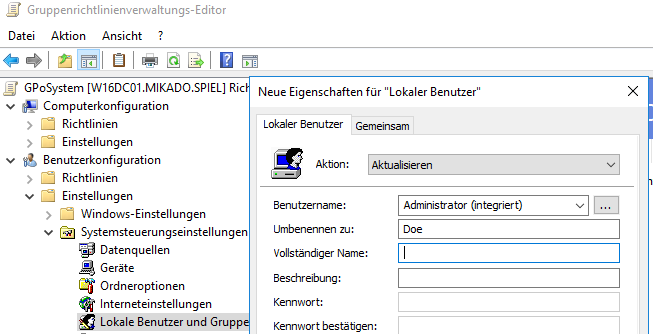
\includegraphics[width=6.3in,height=3.22236in]{figures/image23.png}

Die Umbenennung soll helfen, damit Nutzer oder Schadsoftware das
Administrator Konto schlechter finden können.

\hypertarget{zugriffsrechte}{%
\section{Zugriffsrechte}\label{zugriffsrechte}}

Zugriffsrechte dienen in erster Linie, das System vor ungewollten
Zugriff zu sch\"utzen. Sie sch\"utzen jedoch nicht nur den Computer, sondern
auch das Netzwerk vor Schadsoftware, welche beispielsweise durch USB
Massenspeichern auf den Rechner \"ubertragen werden können.

\hypertarget{zugriff-auf-lokale-laufwerke}{%
\subsection{Zugriff auf Lokale
Laufwerke}\label{zugriff-auf-lokale-laufwerke}}

Damit Benutzer am Rechner keine Viren in das Netzwerk einschleusen
können, sollen Laufwerke, wie auch USB Massenspeicher am Rechner
Deaktiviert werden. Diese Einstellung wird innerhalb der
Gruppenrichtline festgelegt. Damit beispielsweise nicht alle Nutzer von
diesen Anpassungen betroffen sind, kann eine neue Gruppenrichtline
hierf\"ur definiert werden, welche nur an bestimmte Sicherheitsgruppen
zugewiesen werden. Ausgenommen werden hier beispielsweise
Administratoren oder die F\"uhrungsebene.

Um diese Einschränkung festlegen zu können, muss unter
Benutzerkonfiguration \textgreater{} Richtlinie \textgreater{}
Administrative Vorlage \textgreater{} System \textgreater{}
Wechselmedienzugriff folgende Richtlinie aktiviert werden:

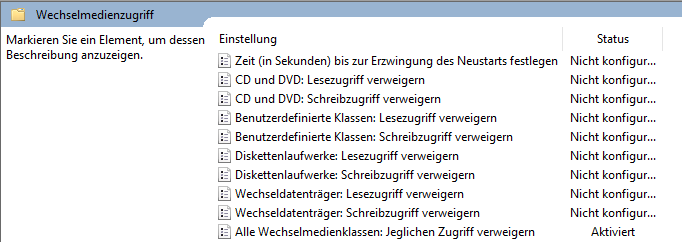
\includegraphics[width=6.3in,height=2.23548in]{figures/image24.png}

Sollte diese Regel aktiviert werden, so sind alle Wechseldatenträger an
diesem Rechner, wo der Benutzer angemeldet ist deaktiviert. Diese Regel
greift, bevor andere Regeln f\"ur spezifische Wechseldatenträger definiert
wurden.

\hypertarget{zugriff-auf-eingabeaufforderung}{%
\subsection{Zugriff auf
Eingabeaufforderung}\label{zugriff-auf-eingabeaufforderung}}

Der Zugriff auf die Eingabeaufforderung sollte im Regelfall nur
deaktiviert werden, falls kein Anmeldeskript oder Skript beim An- oder
Abmelden hinterlegt ist, da dieses andernfalls nicht ausgef\"uhrt werden
kann. Sollte kein Anmeldeskript oder sonstige Skripte vorhanden sein,
die eine Eingabeaufforderung bed\"urfen, kann diese Richtlinie unter
Benutzerkonfiguration \textgreater{} Administrative Vorlage
\textgreater{} System \textgreater{} Zugriff auf Eingabeaufforderung
verhindern aktiviert werden.

Zuweisen von Laufwerken und Druckern, kann ebenfalls \"uber eine
Gruppenrichtlinie festgelegt werden.

\hypertarget{zugriff-auf-systemadministration}{%
\subsection{Zugriff auf
Systemadministration}\label{zugriff-auf-systemadministration}}

Um den Zugriff auf Systemeinstellungen zu verbieten, damit hier keine
Änderungen an dem Computersystem vorgenommen werden kann, wird diese
Konfigurationsmöglichkeit, f\"ur jeden Benutzer deaktiviert. Damit kann
ein Benutzer die Systemsteuerung, sowie Informationen zu Konfiguration
des Computers nicht mehr abrufen oder verändern. Diese Richtlinie kann
innerhalb der Gruppenrichtlinie unter Benutzerkonfiguration
\textgreater{} Administrative Vorlagen \textgreater{} Systemsteuerung
aktiviert werden.

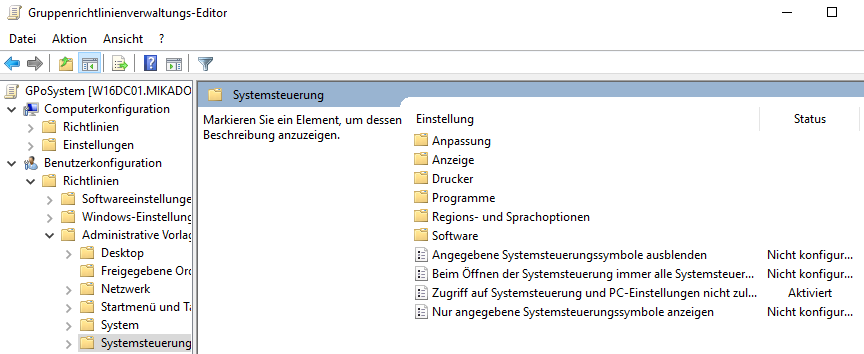
\includegraphics[width=6.3in,height=2.58125in]{figures/image25.png}

\hypertarget{datenaustausch}{%
\section{Datenaustausch}\label{datenaustausch}}

F\"ur den Datenaustausch der Mitarbeitern, sowie Abteilungsleitern, sind
folgende Anforderungen definiert worden:

Die Abteilungsleiter untereinander uneingeschränkt Daten austauschen
können.

Hierzu muss zunächst eine Sicherheitsgruppe \enquote{LGsAbteilungsleiter}
erstellt werden, damit nicht jeder Mitarbeiter einzelnen in die Freigabe
ausgewählt werden muss. Anschließend muss eine Freigabe erstellt werden
\enquote{ExchangeAbt} auf die die Sicherheitsgruppe Lese, sowie
Schreibberechtigung besitzt. Dieses Laufwerk kann nun \"uber eine
Zusätzliche Gruppenrichtlinie an die Abteilungsleitern \"uber die
Sicherheitsgruppe zugewiesen werden.

Die nächste Anforderung ist, dass Abteilungsleitern, Aufträge f\"ur
Mitarbeiter einstellen können, diese die Daten jedoch nur abrufen
können.

Hierzu muss zunächst eine Sicherheitsgruppe f\"ur die Mitarbeiter
\enquote{LGsMitarbeiter} erstellt werden und zusätzlich eine Freigabe, welche
\enquote{Auftraege} lautet. Auf diese Freigabe muss nun die Sicherheitsgruppe
\enquote{LGsAbteilungsleiter} lese, sowie schreibberechtigung besitzen.
Mitarbeiter erhalten hier mit der Sicherheitsgruppe \enquote{LGsMitarbeiter}
nur Leseberechtigung.

Dies kann ebenfalls in umgekehrter Reihenfolge f\"ur Aufträge gemacht
werden, welche Mitarbeiter den Abteilungsleitern lesend zur Verf\"ugung
stellen. Eine zusätzliche Freigabe \enquote{beaAuftraege} wird benötigt.

Die Zuweisung der Laufwerksbuchstaben f\"ur die Clients, kann \"uber eine
separate oder zuvor erstellte Gruppenrichtlinie zugewiesen werden. Die
Richtlinie/Konfiguration ist hierzu unter Benutzerkonfiguration
\textgreater{} Einstellungen \textgreater{} Windows-Einstellungen
\textgreater{} Laufwerkszuordnung \textgreater{} neu

Hinzugef\"ugt werden.

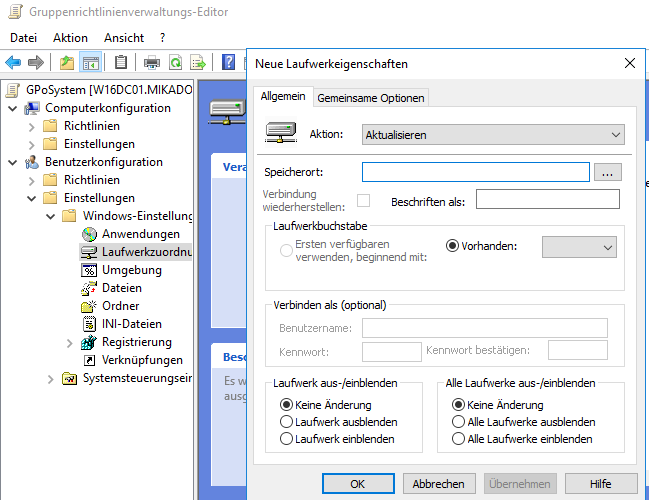
\includegraphics[width=6.3in,height=4.85362in]{figures/image26.png}

Hier hat der Administrator nun die Möglichkeit, den Speicherort f\"ur
diese Freigabe festzulegen. Die Zuweisung der GPo als solches, wird \"uber
die Sicherheitsrichtlinie \enquote{LGsMitarbeiter} und \enquote{LGsAbteilungsleiter}
durchgef\"uhrt.

\chapter{Fazit}

%\appendix

\printglossaries%

\begingroup
\tolerance1000
\emergencystretch0.5em
\printbibliography[heading=bibnumbered]
\endgroup

\chapter{Anhang}

\input{figures.tex}
\FloatBarrier%
\begin{listing}[ht]
  \inputminted[fontsize=\small]{text}{listings/atop.txt}
  \caption{atop ASCII Logausgabe}
  \label{lst:atop}
\end{listing}

\FloatBarrier%
%\begin{center}
  \begin{tabularx}{\textwidth}{p{2.5cm} lX}
  \toprule
    Projekt     & URL                                                   \\
  \midrule
    Puppet      & https://tickets.puppetlabs.com/browse/PA-668          \\
    Puppet      & https://tickets.puppetlabs.com/browse/PUP-7383        \\
    Mcollective & https://tickets.puppetlabs.com/browse/MCO-804         \\
    Grafana     & https://github.com/voxpupuli/puppet-grafana/issues/35 \\
  \bottomrule
\end{tabularx}
\captionof{table}{Gemeldete Bugs in Open Source Projekten}
\label{tbl:fossissues}
\end{center}


\label{pdf:requirements}
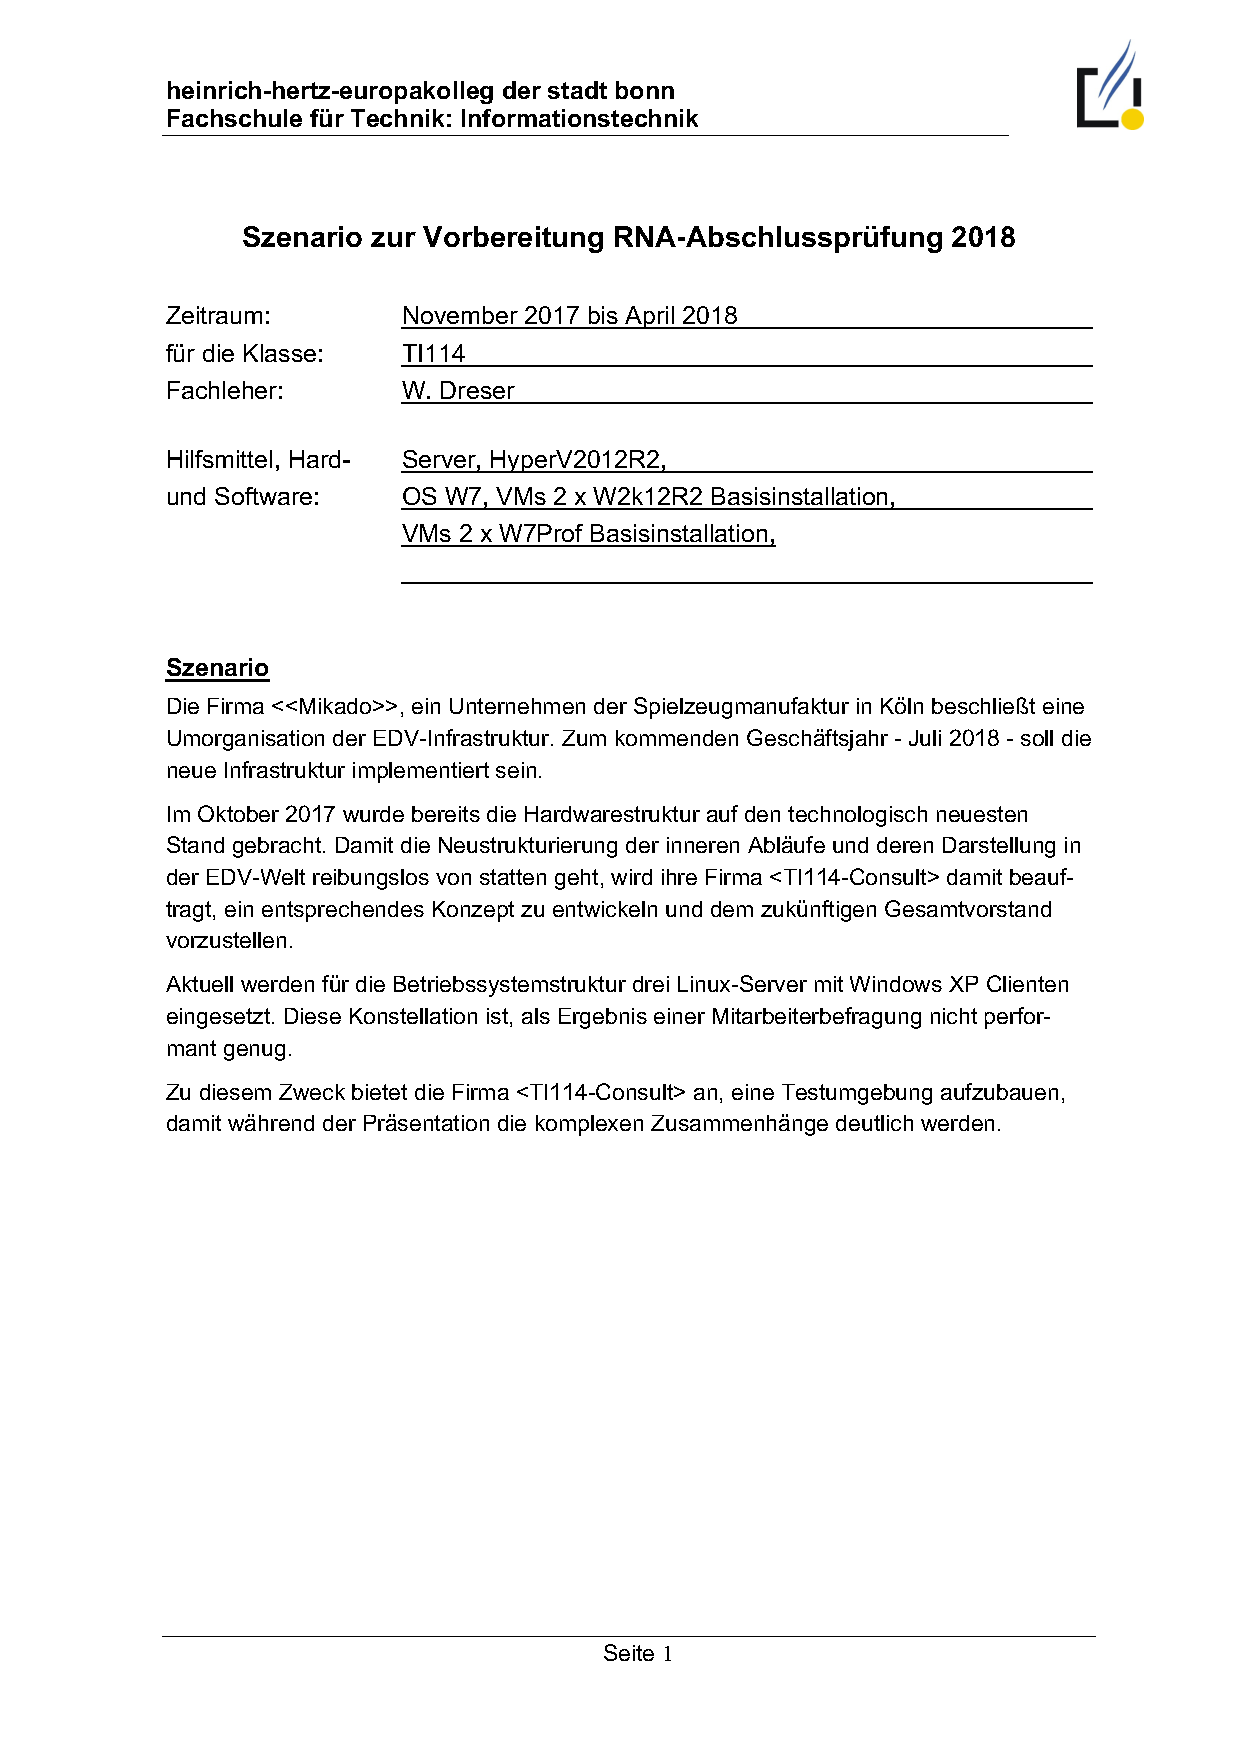
\includepdf[pages=-]{Szenario-TI114-2017.pdf}

\chapter{Erklärung}
Hiermit erklären wir, dass wir die Arbeit selbstständig verfasst und keine
anderen als die angegebenen Quellen und Hilfsmittel benutzt haben. Diese Arbeit
wurde keinem anderen Pr\"ufungsausschuss in gleicher oder vergleichbarer Form
vorgelegt.

\vspace{10ex}
{\centering
\renewcommand{\arraystretch}{0.9}
\begin{tabular}{p{0.25\textwidth}p{0.05\textwidth}p{0.25\textwidth}p{0.05\textwidth}p{0.25\textwidth}}
  \dotfill                    & & \dotfill                      & & \dotfill \\
  \centering\footnotesize{Tim Meusel}& & \centering\footnotesize{Marcel Reuter}& & \centering\footnotesize{Nikolai Luis}%
\end{tabular}
}

%%% Local Variables:
%%% mode: latex
%%% TeX-master: "thesis-de"
%%% End:
